%compiling with XeLaTeX
\documentclass[digital, %colors on
			   %print,  %for printing
			   %twoside, %turn off for digital version
			   openright, %chapter always start on the right page
			   parskip=half,
			   11pt]{mythesis}
			  

%Presets		   
%Personel Data
\title{Quark Spectral Functions from Dyson-Schwinger Equations with Spectral Renormalization}
\author{Mathieu Kaltschmidt}
\date{\today}

%Adding bib
\addbibresource{bib/msc.bib}

%Statements
\newtheorem{statements}{Statements}[chapter]

%Statement environment
\newcommand{\statement}[1]{\stepcounter{statements}\begin{center}
	\textbf{#1}
	\end{center}
}


%Some more packages
\usepackage{epigraph}
\setlength{\epigraphwidth}{.8\textwidth}
\setlength{\epigraphrule}{0pt}

%Useful definitions

\newcommand{\Z}{\mathcal{Z}[J]}
\renewcommand{\S}{\mathcal{S}[\varphi]}
\newcommand{\D}{\mathcal{D}}
\newcommand{\W}{\mathcal{W}[J]}
\newcommand{\cf}[1]{\langle #1 \rangle}



\begin{document}
\pagenumbering{Roman}

%Introductory stuff, abstracts and toc
{\hypersetup{allcolors=black}
%\newgeometry{centering}    
\begin{titlepage}
\begin{center}
		\makeatletter
				\vspace{2cm}
		\Large\textbf{Department of Physics and Astronomy\\
			 University of Heidelberg}
		\vfill
		\normalsize
		Master thesis in Physics\\
		\normalsize
		submitted by\\[0.4cm]
		\Large
		\textbf{\@author}\\
		\normalsize
		born in Herbolzheim, Germany \\ [0.4cm]
		handed in on\\
		\Large
		\textbf{June 15th, 2021}
		\cleardoublepage
		\thispagestyle{empty}
		\vspace{2cm}
		\Large\textbf{Quark Spectral Functions from Dyson-Schwinger Equations with Spectral Renormalization}\\[.4cm]
		\vfill
		\normalsize
		This Master thesis has been carried out by \\ 
		\vspace{3pt}
		\textbf{\@author}  \\ 
		\vspace{3pt}
		at the\\
		\vspace{3pt}
		\textbf{Institute for Theoretical Physics} \\ at the \\\textbf{University of Heidelberg}\\
		\vspace{5pt}
		under the supervision of\\
		\vspace{5pt}
		\textbf{Prof. Dr. Jan M. Pawlowski}\\
		\makeatother
\cleardoublepage
\end{center}
\end{titlepage}} 
%\restoregeometry 

\pagenumbering{Roman}
\begin{center}

	\makeatletter
	\thispagestyle{plain}
	\LARGE\bfseries{\@title} \\
 	\vspace{4mm}
	\large\bfseries{\@author} \\
	\normalfont
	\vspace{4mm}
	\large{May 10th, 2021} \\
	\vspace{2mm}
	\large{Institute for Theoretical Physics \\
		University of Heidelberg } \\
	\makeatother
\end{center}

\normalsize
\noindent This short report summarizes the current state of the art of my Master thesis research carried out as a member of the Strongly Correlated Systems Group at the Institute for Theoretical Physics in Heidelberg  under the supervision of Prof. Jan M. Pawlowski. \\

\noindent  We compute non-perturbative quark spectral functions for QCD in the Landau gauge. The spectral densities $\rho_i$\ are obtained by iteratively solving the corresponding Dyson-Schwinger equation for the quark propagator for a given input gluon spectral function.\\
 %TODO: Describe features of the result in a few sentences
 For the computation of the contributing one-loop quark self energy $\Sigma(p^2)$\ we make use of spectral renormalization, a technique based on dimensional regularization which has been developed recently in our group  \cite{Horak2019, Wink2020, HorakPawlowskiWink2020}. First promising results for the Yang-Mills sector of QCD have successfully proven the power of this method \cite{HorakPapavassiliouPawlowskiWink2021}. With our complementary computations for the matter sector of QCD we aim at contributing to the long term goal of our project line: Obtaining a general understanding of the spectral properties of QCD (at finite temperature and density) and its corresponding  phase diagram.
{
\hypersetup{linkcolor=black}
\tableofcontents  
}
\cleardoublepage


%\setcounter{tocdepth}{1}
\pagenumbering{arabic}

%Main part
	\chapter{Introduction \& Motivation}\label{chap:motivation}
Understanding the properties of Strongly Correlated Quantum Systems is a cornerstone of modern physics research. Experimental and theoretical studies of such systems range from ultracold atoms to the hot phases of the Early Universe and from the non-perturbative infrared sector of Quantum Chromodynamics (QCD) to  ultraviolet completions of the Standard Model of Particle Physics and possible connections to the realization of a theory of Quantum Gravity in Nature.\\
This thesis focuses particularly on the infrared regime of QCD, the theory of strong interactions, describing the physics of quarks and gluons, the fundamental constituents of atomic nuclei. The strong interaction being  one of the four fundamental forces, QCD is embedded in the framework of the Standard Model of Particle Physics, hence is of particular importance for fundamental physics. From a theorist's point of view, the Standard Model is the most general renormalizable field theory with gauge group 
\begin{equation}
	G_{\text{SM}} = SU(3)\otimes SU(2) \otimes U(1),
\end{equation}
three generations of fermions, and a scalar \cite{Hebecker2020}. Here, the pure gauge part of QCD contributes via the non-Abelian $SU(3)$ color group. This description of the gluonic sector in terms of a non-Abelian gauge theory goes back to the pioneering work of Yang and Mills in 1954 \cite{YangMills1954}, hence it is usually referred to as Yang-Mills theory.     \\
Understanding the infrared dynamics of the Yang-Mills sector of QCD is directly linked to the most pressing open questions in QCD, for an overview cf. \cite{Brambilla2014}. Maybe the most prominent example is the phenomenon of confinement, i.\,e. that the theory features a mass gap\footnote{The mathematical proof of the existence of a mass gapped quantum Yang-Mills theory has even been declared as one of the seven Millennium Prize Problems \cite{JaffeWitten2009}.} and that quarks and gluons can only be observed as color-neutral bound states, called hadrons \cite{vonSmekalAlkoferHauck1997, AlkoferVonSmekal2000, LercheVonSmekal2002, FischerMaasPawlowski2008,CyrolFisterMitterPawlowskiStrodthoff2016}. The associated temperature of the so-called confinement-deconfinement transition, i.\,e. the transition between the confined phase and a state of matter called the Quark-Gluon Plasma (QGP), where the deconfined quarks and gluons are the relevant degrees of freedom, has been determined in lattice studies to be of the order of $T\approx 155$ MeV \cite{AokiFodorKatzSzabo2006}. The phenomenologically rich hadron spectrum makes up a large fraction of all observed matter around us and has been subject of many experimental and theoretical investigations during the last decades.\\ Open questions in the matter sector of QCD include for example the understanding of resonant four-quark interactions \cite{Eichmann2020}, directly connected to the beforehand mentioned variety in the hadronic spectrum and spontaneous chiral symmetry breaking \cite{MitterPawlowskiStrodthoff2014}, the mechanism behind mass generation of nucleons from much lighter quarks. This is usually investigated in low-energy effective models such as Nambu-Jona-Lasinio (NJL) or Quark-Meson (QM) models \cite{NambuJonaLasinio1961, Tetradis2003}. \\ 
\begin{figure}[t]
\centering
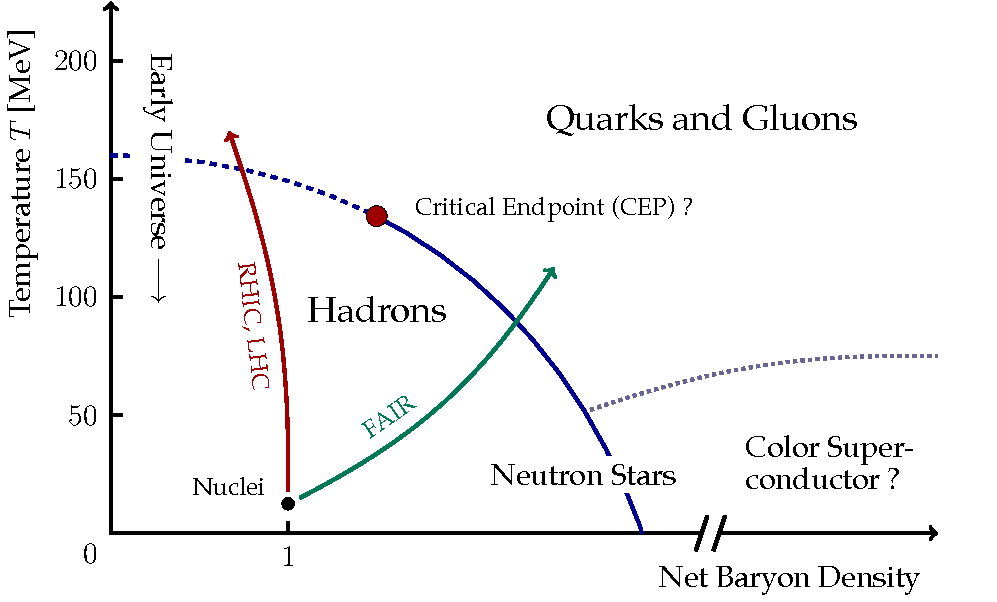
\includegraphics[width=0.8\textwidth]{figs/tikz/qcd_phase_diagram}
\caption[Schematic sketch of the QCD phase diagram.]{Schematic sketch of the QCD phase diagram, inspired by the graphic provided by the GSI/Darmstadt. The dashed blue curve signals a second order phase transition, the solid blue curve the (possible) first order transition regime. The red and green lines indicate the respective areas of the diagram that are tested by experiments at the moment or in the near future, cf. \cite{RHIC, LHC, FAIR, NICA}.}\label{fig:phase_diagram}
\end{figure}
\hspace{-0.5em}Another major task is to obtain a comprehensive understanding of the full QCD phase diagram at finite temperature and baryon density  \cite{Wink2020, BraunHaasMarhauserPawlowski2009,FuPawlowskiRennecke2019}, cf. \figref{fig:phase_diagram} for a schematic overview. Current debates focus for example on the question whether there exists a critical endpoint (CEP) \cite{AokiFodorKatzSzabo2006}. \\
On the technical side, our theoretical understanding of the non-perturbative sector of QCD from first principles has greatly improved during the last decades, mainly due to complementary efforts and advances in the application  of lattice techniques \cite{Philipsen2007, deForcrand2010} and  Functional Methods such as the Functional Renormalization Group (FRG), cf. \cite{Wetterich1992, Pawlowski2005, Dupuis2020} for general reviews, and \cite{NPgaugeLecture} for various applications in QCD (and Gravity), Bethe-Salpeter equations \cite{BetheSalpeter1951}, or Dyson-Schwinger equations (DSEs) \cite{Dyson1949, Schwinger1951}. The latter one will be the tool of our choice throughout this work. Earlier studies of the infrared regime of QCD using DSEs were put forward for example in \cite{Fischer2006,Fischer2019, Maris2003, RobertsWilliams1994}.\\
Of course, there have also been many advances on the experimental side, where the phase diagram is usually studied in the context of relativistic heavy-ion collisions at collider facilities such as the Relativistic Heavy-Ion Collider (RHIC) at the Brookhaven National Lab \cite{RHIC} and the Large Hadron Collider (LHC) at CERN in Geneva \cite{LHC} and in the near future at FAIR/GSI in Darmstadt \cite{FAIR} and NICA in Dubna \cite{NICA}. \\
Nevertheless, it is far from trivial to map measured signatures directly to certain points in the phase diagram. This is due to the fact, that the phase diagram is associated with equilibrium, which is definitely not realized in the initial stages of heavy-ion collisions. Understanding the thermalization process, i.\,e. the stage at which the system approaches thermal equilibrium, is therefore key to be able to connect the measured signatures to theoretical predictions. But this is still a subject of ongoing research efforts, cf. \cite{Blaizot2012, Blaizot2016, Wolschin2020, SchlichtingTeaney2019}.\\
To conclude this overview, we should remark, that all these different methods suffer from technical limitations and are therefore only applicable in specific regions of the phase diagram. Certainly, one should not forget the contributions from perturbation theory (PT) that had great impact on the development of the theory, cf. \cite{EllisGeorgiMachacekPolitzerRoss1979,BernardGolterman1992}, but in in the infrared sector, PT is not applicable since it is usually based on expansions in terms of small coupling constants, which is in conflict with the observation of asymptotic freedom, i.\,e. that the gauge coupling rises extremely quick in the infrared and tends to zero in the ultraviolet. This prediction earned Gross, Politzer and Wilczek the 2004 Nobel Prize in Physics \cite{Politzer1973, GrossWilczek1973}. Lattice computations, where the idea is to discretize the continuum theory and restore the physical continuum limit by extending the lattice size and lowering the grid spacing, make solid predictions for small and vanishing chemical potential. In the region $\mu/T\gtrsim 1$, the infamous sign-problem hinders predictability \cite{Philipsen2007, deForcrand2010}. The application of functional methods is in general not affected by such inherent problems, but rather by limitations in computing power and analytic feasibility of the conducted computations. This will of course improve in the future with the ongoing developments in hardware and computer-algebra systems.\\
A pivotal ingredient in the study of Strongly Correlated Systems are real-time correlation functions since they allow us to access the real-time dynamics of the theory at hand. In the context of QCD this includes for example transport phenomena relevant in the hydrodynamical description of heavy-ion collisions as outlined above, cf. \cite{AyikNorenbergWolschin1977, Xu2019}.\\  
Despite the beforehand mentioned advances in the field, the direct computation of these real-time quantities has turned out to pose several problems, i.\,e. results can only be obtained employing specific approximation schemes. We want to tackle this challenging task by making use of the recently developed technique of Spectral Renormalization \cite{Horak2019, Wink2020, HorakPawlowskiWink2020}, allowing for the direct computation of real-time correlation functions from their respective spectral representations, based on the gauge-invariant dimensional regularization scheme.\\
In this thesis we will focus on the real-time properties of QCD, or to be more precise, on the computation of spectral functions for the quark sector and the analytic properties of the associated correlation functions, since they provide the information needed for first principle investigations of the dynamical properties of the theory.\\

 The structure of this work is as follows. In  \chapref{chap:methods} we lay the foundation for the field theoretical conventions. We employ the functional methods needed for our treatment of non-perturbative QCD including the Dyson-Schwinger equation as the central functional relation in the context of our work. A discussion of the spectral properties of the theory in terms of the K\"all\'{e}n-Lehmann spectral representation of correlation functions completes our introduction to non-perturbative quantum field theory. \chapref{chap:qcd} provides the background knowledge on the quantization of general non-Abelian gauge theories and the special case of $SU(N_c)$ Yang-Mills theory, the underlying gauge theory of QCD. Subsequently, the fermionic quark sector of QCD is discussed and the respective Dyson-Schwinger equations are presented. A detailed presentation and assessment of the methodology and our main results follow in \chapref{chap:results}. Our findings are then summarized in \chapref{chap:conclusion} and an outlook for future investigations is given. \\
The interested reader can find the technical details of the conducted calculations in \appref{chap:appendixA} and \appref{chap:appendixB} respectively. Additional comments on the numerical implementation in Mathematica can be found in \appref{chap:appendixC}.\\
 Throughout this thesis we use natural units such that $\hbar = c  \equiv 1$ and work in Euclidean spacetime  $g_{\mu\nu}=\delta_{\mu\nu}$. Einsteins sum convention is implicitly understood: Whenever an index appears twice in a single term, summation of that term over the whole index range is implied. As usual, greek indices refer to some $d$-dim. spacetime coordinates, ranging from $0$ to $d-1$, i.\,e. $x^{\mu} = (x^0, x^1, \cdots, x^{d-1})$. Vectorial quantities are typeset in boldface. Unless stated otherwise, we work in $d=4$ spacetime dimensions.
	
	\chapter{Functional Methods in QFT}\label{chap:methods}
This chapter introduces a treatment of quantum field theory using functional methods. The main goal is to become familiar with the concepts and the formal and diagrammatic notation used throughout this work and to derive the Dyson-Schwinger Equations \cite{Dyson1949, Schwinger1951} in a simple scalar theory setting. To conclude this formal introduction to the subject, we will introduce the K\"all\'{e}n-Lehmann spectral representation for correlation functions \cite{Kallen1952, Lehmann1954}. Concerning notational conventions and for most parts of the presented derivations we closely follow \cite{NPgaugeLecture}.

\section{Generating Functionals and Dyson-Schwinger Equations}
Consider a theory setting of $N$ real scalar fields $\varphi_a(x), a \in \{1,\dots,N\}$ in $d$-dimensional Euclidean space described by the action functional
\begin{equation}
S[\varphi]=\int_{x} \frac{1}{2}\left(\partial_{\mu} \varphi\right)^{2}+\frac{m^{2}}{2} \varphi^{2}+\frac{\lambda_4}{4 !} \varphi^{4}, \label{eqn:phi4_action}
\end{equation}
and the corresponding partition sum in presence of external sources $J_a(x)$ 
\begin{align}
	Z[J] = \frac{1}{\mathcal{N}} \int \D\varphi \operatorname{e}^{-S[\varphi] + J\cdot\varphi},
	\label{eqn:partition}
\end{align}
with some normalization constant $\mathcal{N}$ and the usual path integral measure 
\begin{equation}
\mathcal{D}\varphi = \prod_{a=1}^{N} \dd \varphi_a.
\end{equation} 
In this notation the scalar product sums over field components and integrates over all space,
\begin{align}
	J\cdot\varphi = \int_x J_a(x) \ \varphi_a(x) = \int_p \tilde{J}_a(p) \ \tilde{\varphi}_a(p),
\end{align}
with the integral conventions
\begin{align}
\int_x = \int_{\mathbb{R}^d} \dd^d x \qquad \text{and} \qquad \int_p = \int_{\mathbb{R}^d} \frac{\dd^d p}{(2\pi)^d}.	
\end{align}

The partition sum $Z[J]$ is called a \textit{generating functional}. Field expectation values are computed via functional derivatives of the partition sum,
\begin{align}
	\phi := \cf{\varphi} = \eval{\frac{1}{Z}\frac{\delta Z}{\delta J}}_{J=0} = \int \D\varphi \ \varphi \ \operatorname{e}^{-S[\varphi] + J\cdot\varphi}.
\end{align}
This is generalized straightforwardly to higher order correlation functions, that are obtained as the $n$-th moments of $Z[J]$,
\begin{align}
\cf{\varphi(x_1) \cdots \varphi(x_n)} := \cf{\varphi^n} = \frac{1}{Z}\eval{\frac{\delta^n Z}{\delta^n J}}_{J=0} = \int \D\varphi \ \underbrace{\varphi_1 \cdots \varphi_n}_{=: \ \varphi^n} \ \operatorname{e}^{-S[\varphi] + J\cdot\varphi}.
\end{align}

\begin{figure}[t]
\centering
	\begin{align*}
\cf{\varphi^4} \hspace{1em}= \hspace{-1em}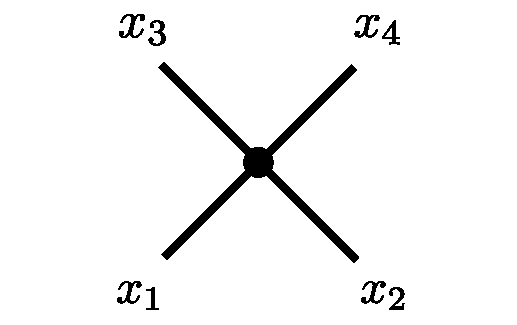
\includegraphics[scale=0.45, valign=c]{figs/diagrams/correlations/connected_01} \hspace{-1em}+ \hspace{-1em}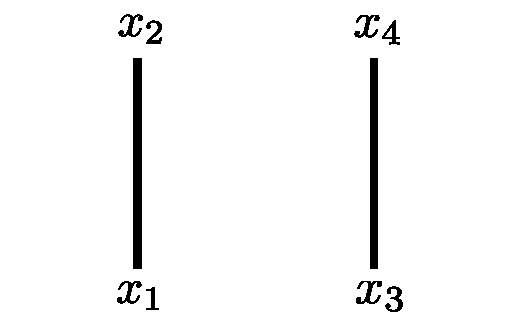
\includegraphics[scale=0.45, valign=c]{figs/diagrams/correlations/disconnected_01} \hspace{-1em}+\hspace{-1em} 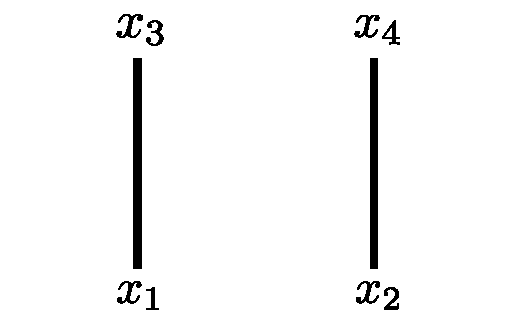
\includegraphics[scale=0.45, valign=c]{figs/diagrams/correlations/disconnected_02} \hspace{-1em}+\hspace{-1em} 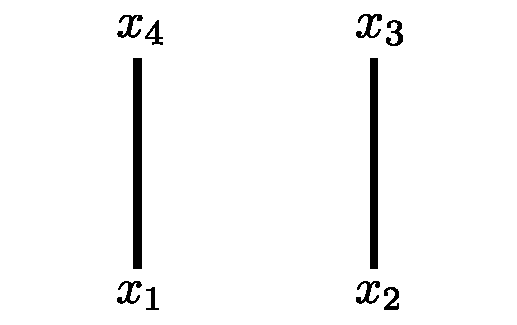
\includegraphics[scale=0.45, valign=c]{figs/diagrams/correlations/disconnected_03}
	\end{align*}
\caption[Visualization of the connected and disconnected parts contributing to the 4-point function in scalar theory.]{Visualization of the connected and disconnected parts contributing to the 4-point function in scalar theory \cite{QFTNotesFloerchingerWetterich}. The relevant contribution to the scattering process is already contained in the connected diagram.}
\label{fig:connected_correlators}
\end{figure}

From an axiomatic viewpoint, the Whightman reconstruction theorem tells us, that the complete set of corresponding $n$-point correlation functions defines the respective quantum field theory entirely and uniquely \cite{Wightman1956}. This explains why the computation of the correlation functions is a task of major importance for the theoretical understanding of a certain QFT. \\
Nevertheless, the correlation functions derived as above contain redundant information, cf. \figref{fig:connected_correlators}. For a more efficient description of the theory in terms of only the \textit{connected} correlation functions, we define the \textit{Schwinger functional} $W[J]$ as the logarithm of $Z[J]$,  
\begin{align}
W[J] = \ln Z[J].
\label{eqn:Schwinger}
\end{align}
It is the generating functional for the connected correlation functions. The normalization factor $\mathcal{N}$, introduced in \eqref{eqn:partition} enters here as an additive constant, which drops out for all higher order correlation functions, except for the 0-point function. This term is connected to the thermodynamic quantities of the system and becomes important, when external parameters such as temperature, volume or the chemical potential are tuned. Nevertheless, in general we are only interested in correlation functions with $n\geq 1$ and therefore we will not focus on this term explicitly in the following.\\
To understand how this redefinition subtracts the disconnected parts of the correlation functions, consider for example the connected 2-point function $W^{(2)}_{ab}(x_1,x_2) = W^{(2)}_{\alpha\beta}$\footnote{To save on notation, we introduce collective indices $\alpha = (x_1,a)$ or $(q_1,a)$ in momentum space.}, correlating the field $\varphi_a$ at spacetime point $x$ with the field $\varphi_b$ at $y$,
\begin{equation}
\begin{aligned}
	W^{(2)}_{\alpha\beta} &= \frac{\delta^2W[J]}{\delta J_{\alpha}\delta J_{\beta}} = \frac{\delta}{\delta J_{\alpha}}\left(\frac{1}{Z}\frac{\delta Z}{\delta J_{\beta}}\right) = \frac{1}{Z}\left(\frac{\delta^2Z}{\delta J_{\alpha}\delta J_{\beta}}\right) - \frac{1}{Z^2}\left(\frac{\delta Z}{\delta J_{\alpha}}\right)\left(\frac{\delta Z}{\delta J_{\beta}}\right)\\[0.5em]
				&= \cf{\varphi_{\alpha}\varphi_{\beta}} - \phi_{\alpha}\phi_{\beta} = \cf{\varphi_{\alpha}\varphi_{\beta}}_{\mathrm{c}}. 
\end{aligned}
\label{eqn:G_connected}						
\end{equation}
This quantity is known as the propagator, the central object of interest in functional approaches to QFT, 
\begin{equation}
	G(x_1,x_2) := W^{(2)}(x_1,x_2).
\end{equation}
It is possible to make computations even more efficient, because $W[J]$ still contains redundant information. Connected correlation functions can be separated into so-called \textit{one-particle irreducible} (1PI) and \textit{reducible} ones. In terms of diagrams, the 1PI correlation functions are those, whose corresponding Feynman diagrams can \textit{not} be separated into two disconnected parts by cutting a single internal line, cf. \figref{fig:1PI_correlators}. If the diagram is reducible in this sense, it can be expressed by multiplying the two disconnected parts with the cut propagator. The disconnected parts are then of the same or lower loop-order and are therefore already included.\\
The generating functional for the  1PI correlation functions, the \textit{effective action} $\Gamma$, is obtained from the Schwinger functional via a Legendre transformation, 
\begin{equation}
	\Gamma[\phi]=\sup _{J}\left\{\int_{x} J(x) \phi(x)-W[J]\right\}=\int_{x} J_{\mathrm{sup}}(x) \phi(x)-W\left[J_{\mathrm{sup}}\right],
\label{eqn:Def_Gamma}
\end{equation}
where $J_{\mathrm{sup}}$ has to be understood as a field-dependent current $J_{\mathrm{sup}}[\phi]$. In the following, we will drop the subscript, its meaning is implicitly understood. Note, that the effective action depends on the expectation value $\phi$ instead of the full fluctuating fields $\varphi$.

\begin{figure}[t]
\centering
\hfill
\begin{subfigure}{0.4\textwidth}
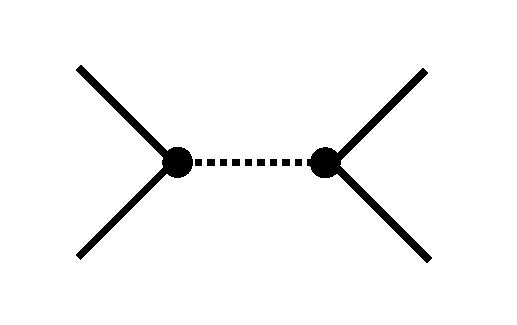
\includegraphics[scale=0.55, valign=c]{figs/diagrams/correlations/connected_02} 
\end{subfigure}
\hfill
\begin{subfigure}{0.4\textwidth}
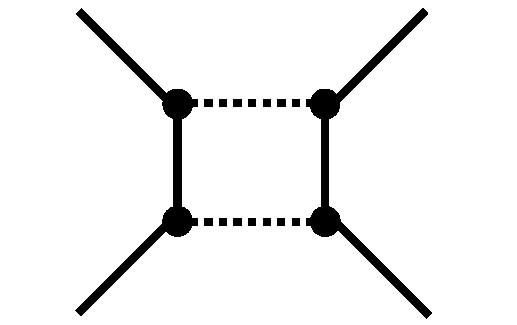
\includegraphics[scale=0.55, valign=c]{figs/diagrams/correlations/1PI} 
\end{subfigure}
\hfill

\caption[Reducible and 1PI contribution to the connected 4-point function in Yukawa theory.]{Reducible (left) and 1PI contributions (right) to the connected 4-point function in Yukawa theory \cite{QFTNotesFloerchingerWetterich}.}
\label{fig:1PI_correlators}
\end{figure}

The quantum equation of motion derived from $\Gamma$ reads
\begin{align}
	J(x) = \frac{\delta\Gamma[\phi]}{\delta\phi(x)}.
	\label{eqn:quantum_eom}
\end{align}
It allows us to understand the dynamics of field expectation values, taking the effects of all quantum fluctuations into account.
From a physical point of view, the effective action $\Gamma$ is the quantum analogue of the classical action $S$. The underlying symmetries of the classical action are in general still present in the effective action.\\
In terms of the effective action, higher order correlation functions are again obtained by performing functional derivatives, but now with respect to the mean field $\phi$,
\begin{align}
	\Gamma^{(n)}[\phi]\left(p_{1}, \ldots, p_{n}\right)=\frac{\delta^{n} \Gamma[\phi]}{\delta \phi\left(p_{1}\right) \cdots \delta \phi\left(p_{n}\right)}.
\end{align}
Here we presented the momentum space expression. The field-dependent propagator derived from the effective action is now given by the \textit{inverse} of the 1PI 2-point function:
\begin{equation}
	G[\phi](p,q) = \frac{1}{\Gamma^{(2)}}[\phi](p,q).
\end{equation}
The path integral measure of the generating functional is invariant under field independent spacetime translations $\phi(x) \rightarrow \phi(x) + \Lambda(x)$ and so are the respective correlation functions. The corresponding symmetry identity derived from this is given by
\begin{equation}
\frac{\delta \Gamma[\phi]}{\delta \phi(x)}=\frac{\delta S[\phi]}{\delta \varphi(x)}\left[\varphi=G \cdot \frac{\delta}{\delta \phi}+\phi\right]. \label{eqn:DSE}
\end{equation}
\begin{figure}[t]
\centering
\begin{subfigure}{0.3\textwidth}
	\begin{align*}
G \hspace{0.5em}= 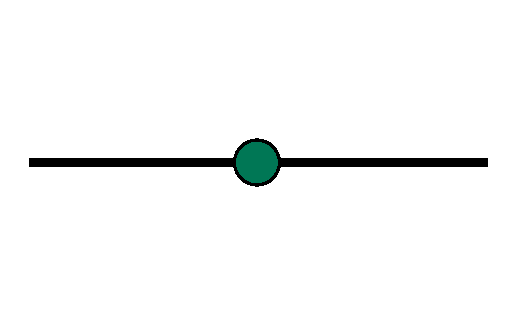
\includegraphics[scale=0.4, valign=c]{figs/diagrams/notation/full_propagator}
	\end{align*}
	\subcaption{Full propagators.}
\end{subfigure}
\hfill
\begin{subfigure}{0.3\textwidth}
	\begin{align*}
S^{(n)} = \hspace{-0.5em}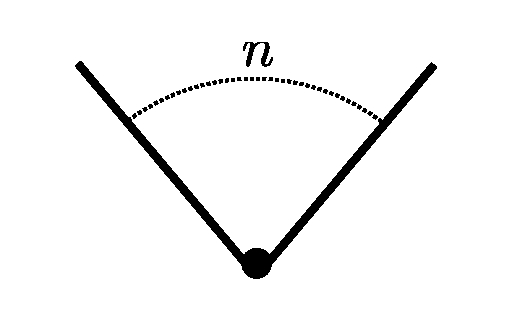
\includegraphics[scale=0.4, valign=c]{figs/diagrams/notation/classical_vertices}
	\end{align*}
	\subcaption{Bare $n$-point vertices.}
\end{subfigure}
\hfill
\begin{subfigure}{0.3\textwidth}
	\begin{align*}
\Gamma^{(n)} = \hspace{-0.5em} 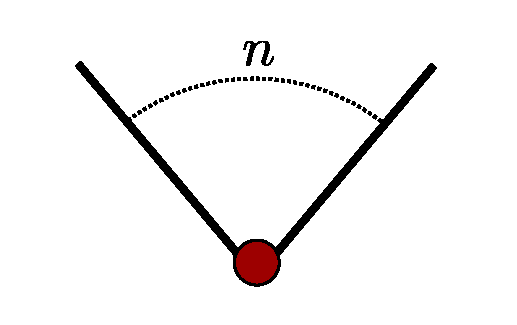
\includegraphics[scale=0.4, valign=c]{figs/diagrams/notation/full_vertices}
	\end{align*}
	\subcaption{Full $n$-point vertices.}
\end{subfigure}
\caption{Overview of the diagrammatic notation used throughout this work.}
\label{fig:notation}
\end{figure}\noindent 
This is the famous \textit{Dyson-Schwinger equation} (DSE), the central functional relation in the context of our work. The DSE therefore establishes a relation between the quantum and the classical equations of motion via the shift independence of the path integral measure. More formal derivations can for example be found in  \cite{NPgaugeLecture, AlkoferVonSmekal2000}. Here, $S[\phi]$ is the classical action of the theory at hand and
\begin{equation}
	G\cdot\frac{\delta}{\delta\phi} = \int\frac{\dd^dq}{(2\pi)^d}\ G(p,q)\frac{\delta}{\delta\phi} .
\end{equation}
This explains how we can extract the correlation functions from the DSE, i.\,e. by taking functional derivatives of equation (\ref{eqn:DSE}). The two-point function is therefore obtained by taking a single field derivative.\\
The DSE admits a diagrammatical representation in terms of full and classical propagators and vertices, respectively. The notational conventions we choose to work with throughout this thesis are displayed in \figref{fig:notation} at the beginning of the last page.\\
To give an explicit example, consider the master DSE for the scalar $\phi^4$-theory described by the action in (\ref{eqn:phi4_action}) obtained from (\ref{eqn:DSE}):
\begin{equation}
\Gamma^{(1)}[\phi]=S^{(1)}[\phi]+\frac{\lambda_{4}}{2!}\ G \cdot \phi-\frac{\lambda_{4}}{3 !}\ G \cdot\left(G \cdot \Gamma^{(3)} \cdot G\right),\label{eqn:masterDSE_scalar1}
\end{equation}
whose diagrammatic representation is displayed in \figref{fig:masterDSE_scalar}.
\begin{figure}[t]
	\centering
	\begin{align*}
	\hspace{-25 pt} 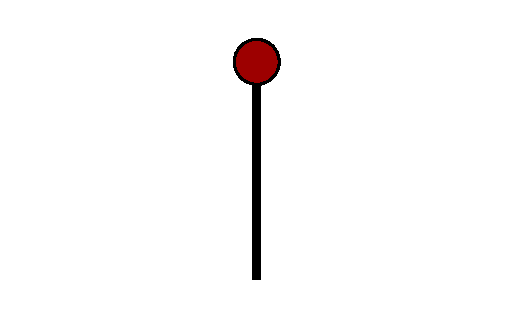
\includegraphics[scale=0.5, valign=c]{figs/diagrams/masterDSE/d_gamma} \hspace{-30 pt}=\hspace{-30 pt} 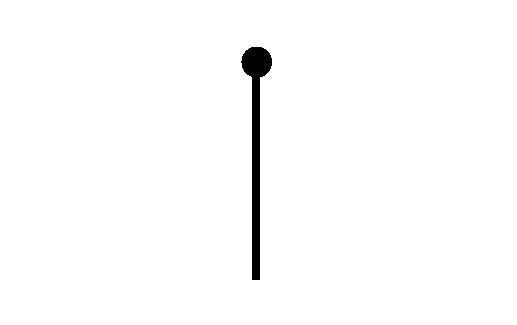
\includegraphics[scale=0.5, valign=c]{figs/diagrams/masterDSE/d_S} \hspace{-30 pt}+\hspace{20pt}\mathlarger{\frac{1}{2}} \hspace{-20 pt}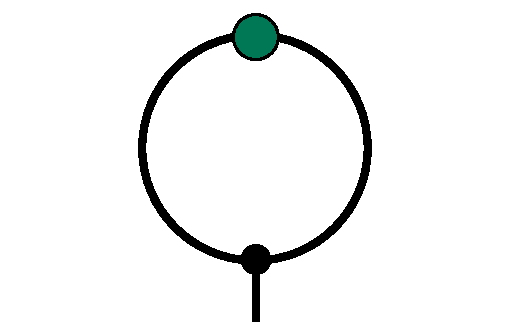
\includegraphics[scale=0.5, valign=c]{figs/diagrams/masterDSE/one_loop} \hspace{-20 pt}-\hspace{20pt} \mathlarger{\frac{1}{6}} \hspace{-20 pt}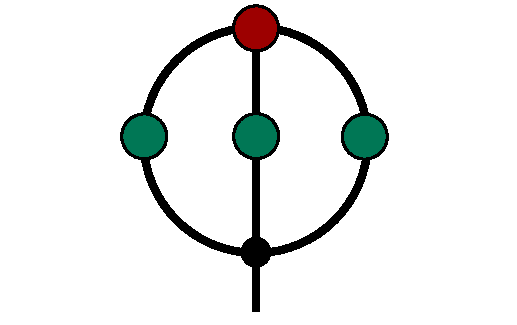
\includegraphics[scale=0.5, valign=c]{figs/diagrams/masterDSE/two_loop}
	\end{align*}
	\caption{Diagrammatic representation of the master DSE in scalar theory (\ref{eqn:masterDSE_scalar1}).}\label{fig:masterDSE_scalar}
\end{figure}

\section{K\"all\'{e}n-Lehmann Spectral Representation}
When applying functional methods such as the DSE in non-perturbative calculations involving loop corrections, the \enquote{classical} momentum scaling
\begin{equation}
	G(p)\sim\left(p^2+m^2\right)^{-1},
\end{equation}
of the propagators for some (possibly vanishing) mass scale $m$ is usually modified. This subtlety can cause severe complications in analytical and numerical computations. A rather simple approach to circumvent this  is provided by the K\"all\'{e}n-Lehmann (KL)  spectral representation \cite{Kallen1952, Lehmann1954} of the propagator, which can be derived from a completeness relation for zero momentum states of the theory, cf. \cite{QFTNotesPawlowskiJaeckel} for a detailed derivation.\\
 The KL representation allows us to recast the propagator in terms of a spectral integral over the respective spectral density (or spectral function) $\rho(\lambda^2)$ with spectral parameter $\lambda$ as follows:
\begin{align} 
G(p)=\int_{0}^{\infty} \frac{\dd \lambda^2}{\pi} \frac{\rho(\lambda^2)}{p^{2}+\lambda^{2}}. \label{eqn:KL_rep}
\end{align}
This can be interpreted as an integral over classical free propagators of a particle with squared mass $\lambda^2$ weighted by the spectral density $\rho(\lambda)$, or for the case of asymptotic states, as probability density for the transition to an excited state with energy $\lambda$. The spectral density $\rho(\lambda)$ encodes all the information about the energy spectrum of the theory.\\
The existence of a spectral representation has been discussed for decades in axiomatic approaches to QFT, cf. \cite{Wightman1965}. This poses strong conditions on the analytic structure of the propagator and imposes tight restrictions on its functional space.\\ Throughout this work, we implicitly assume its existence and in addition a cross-check to benchmark our results is always given by the comparison of the analytical result for the Euclidean propagator with the result from \eqref{eqn:KL_rep} for the computed spectral function. \\
Concerning a mathematical interpretation, the spectral function arises as the set of non-analyticities of the propagator, whose locations in the complex plane are restricted by Cauchy's theorem, cf. \figref{fig:cauchy}.\\
\begin{figure}[t]
	\centering
	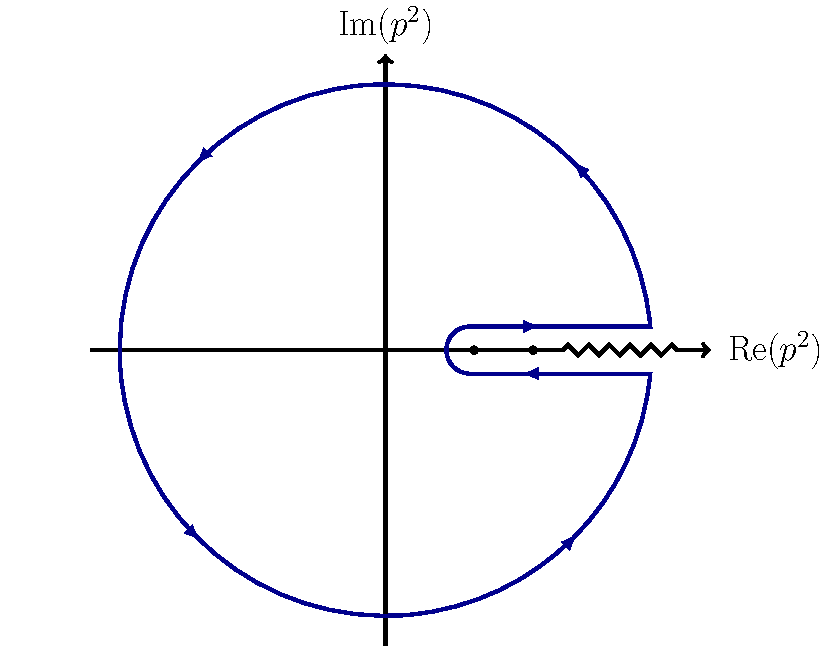
\includegraphics[width=0.6\textwidth]{figs/tikz/contour}
	\caption[Illustration of the analytic structure of an example propagator for a scalar theory featuring a 2-particle bound-state.]{Illustration of the analytic structure of an example propagator for a scalar theory featuring a 2-particle bound-state. The contour is chosen in such a way that all the non-analyticities of the propagator are excluded and corresponds to the evaluation of \eqref{eqn:KL_rep} using Cauchy's theorem. The visualization is inspired by \cite{JiaPennington2017}.} 
	\label{fig:cauchy}
\end{figure}\noindent
From this, an inverse relation between the retarded propagator and the spectral function can be derived, cf. \appref{chap:appendixB} for a detailed derivation. It reads
\begin{equation}
	\rho(\omega, \abs{\mathbf{p}}) = 2 \operatorname{Im}\left[G\left(-i(\omega + i0^+), \abs{\mathbf{p}}\right)\right], \label{eqn:specfunc_relation}
\end{equation}
with $\omega$ being the zero component of the real-time momentum and $0^+$ has to be understood as taking the limit $\varepsilon\rightarrow 0$ from above. This relation is of particular importance, since we will use it later on to extract the spectral function from the computed retarded propagator.\\
 Note, that in this instance, the spectral function is expressed as a function of a linear argument in contrast to the definition in \eqref{eqn:KL_rep}, which is the convention we choose to work with for the remainder of this work. Imposing Lorentz invariance usually enforces the propagator to be a function of $p^2$ and therefore the same must hold for the spectral function. Nevertheless, symmetry arguments for the analytic structure of the propagator in the complex plane allow for a change of variables $\dd\lambda^2 \rightarrow \lambda\ \dd\lambda$.\\
Following the same line of arguments, we do not need to consider the spatial momentum dependence explicitly since for vacuum QFTs all kinematic information can be restored from Lorentz transformations. Hence, we will drop the explicit dependency for the remainder of this work.  \\ 
\begin{figure}[t]
\centering
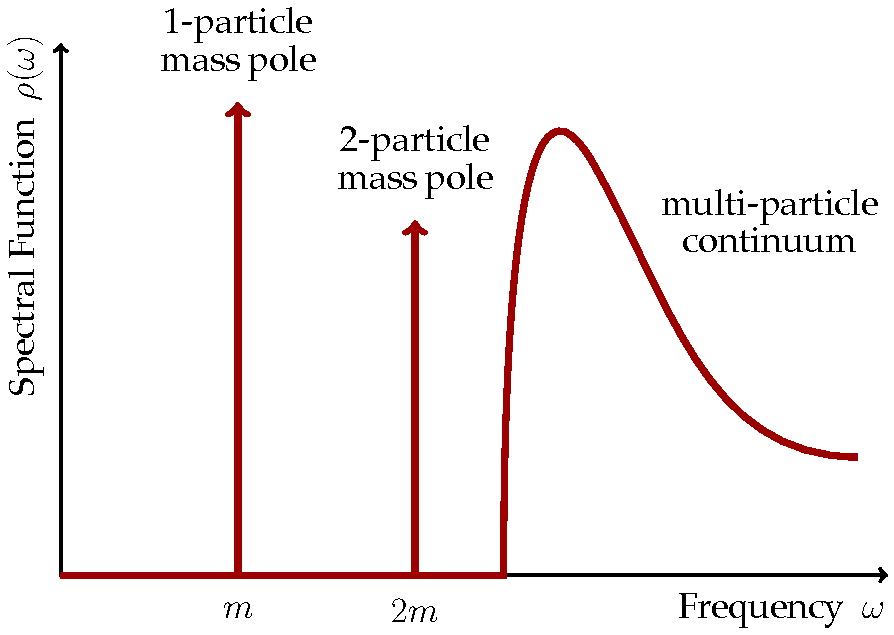
\includegraphics[width=0.6\textwidth]{figs/tikz/scalar_spec_func}
\caption[Shape of a typical spectral function of a scalar theory.]{Shape of a typical spectral function of a scalar theory. The isolated poles of the propagator show up as delta peaks in the spectral function. The continuous tail is generated by branch cuts. The visualization is inspired by \cite{Horak2019}.}\label{fig:scalar_spec_func}
\end{figure}\noindent
From equations (\ref{eqn:KL_rep}) and (\ref{eqn:specfunc_relation}) it follows straightforwardly, that all non-analycities of the propagator are restricted to the real momentum axis. This allows us to split the spectral function into pole contributions and a continuous (scattering) part generated by branch cuts, i.\,e.
\begin{equation}
	\rho(\lambda) =\sum\limits_{i} \frac{\pi R_i}{2\lambda}\ \delta(\lambda-m_i) + \rho_{\mathrm{cont}}(\lambda). \label{eqn:split}
\end{equation}
Here, the $R_i$ are the residues associated to the respective poles at $m_i$.
From this ansatz, the spectral function reproducing the classical propagator is simply obtained from equation (\ref{eqn:split}) by setting $R_1 = 1$, $R_{i>1} = 0 $ and $\rho_{\mathrm{cont}}=0$. An examplary spectral function in the context of a scalar theory is visualized in \figref{fig:scalar_spec_func}.\\
Concerning its probabilistic interpretation, one would expect the spectral density to be positive semi-definite, and for the case of scalar theory considered here, this is indeed true. The following summation rule holds:
\begin{equation}
	\int_0^{\infty}\frac{\dd\lambda}{\pi} \lambda\rho(\lambda) = 1.
\end{equation}
This picture might change for gauge theories, and especially for QCD, since the spectral functions we are interested in, are not spectral functions of asymptotic states and hence not observables. Nevertheless, it is expected that \eqref{eqn:specfunc_relation} is still true. Specifically for QCD, there exists a so-called superconvergence relation \,
\begin{equation}
	\int_0^{\infty}\frac{\dd\lambda}{\pi} \lambda\rho_A(\lambda) = 0.
\end{equation}
This relation makes positivity violation even necessary! On the technical side, a frequently occurring problem is the observation of (possibly) existing complex-conjugated poles, which would be in contradiction with the assumptions made by axiomatic QFT as discussed before.  For further details, cf. \cite{Lowdon2015}. \\
To conclude this section we again want to emphasize that working with spectral representations can facilitate computations a lot, allows for the application of perturbative techniques and can be easily implemented in calculations, as we will see later. Following the recent progress in the pure gauge sector of QCD, we want to dedicate this work to the study of the spectral properties of the matter sector of QCD, which in the end might be the key to access and predict macroscopic observables of QCD such as bulk and shear viscosities.




	\chapter{Quantum Chromodynamics}\label{chap:qcd}
Quantum chromodynamics, the theory of strong interactions, was developed on the basis of scattering experiments that showed the existence of an internal $SU(3)$-symmetry and related (color) charges \cite{NPgaugeLecture} and has been subject to intense research over the last decades. \\
This chapter serves as an introduction to the theoretical formalism behind QCD, most of the treated subjects are textbook knowledge on the level of an advanced QFT course, cf. \cite{NPgaugeLecture, QFTNotesFloerchingerWetterich, QFTNotesPawlowskiJaeckel, PawlowskiPlehnQCD} for lecture notes  or \cite{Muta2010, PeskinSchroeder1995, ItzyksonZuber1980, Thomson2013, Georgi1999} for very detailed textbooks.\\
 Note, that we do not aim to provide a complete introduction to the subject but rather focus on the non-perturbative aspects of the theory to make the reader familiar with the concepts required for a general understanding of the conducted calculations.\\
We will briefly recap the most important steps in the quantization of general non-Abelian gauge theories, introduce the superfield formalism to condense our notation and derive the actions for pure Yang-Mills theory and QCD. We conclude our discussion by presenting the Dyson-Schwinger equations for the gluon, ghost and quark propagators, respectively,  as they are the central functional relations in the context of our work.\\
Concerning notational conventions we again closely follow \cite{NPgaugeLecture} and \cite{Cyrol2017}.


\section{Non-Abelian Gauge Theories and Yang-Mills Theory}\label{sec:yang_mills}
Compared to Abelian theories such as Quantum Electrodynamics (QED) with gauge group $U(1)$ related to the electric charge, the underlaying gauge theory of QCD, $SU(3)$ Yang-Mills theory, is self-interacting and hence already non-trivial on the classical level. The quantization of non-Abelian gauge theories has to be treated very carefully. In the subsequent section we will go through this process and fix our notation.                                                                                                                                                                                                                                                                                                                                                                                                                                                                                                            
\subsection{General Concepts and the Yang-Mills Action}
In general, Lagrangians of physical quantum field theories are constructed such that they are invariant under (gauge) transformations of the respective gauge group. This general requirement and the assumption of minimal coupling leads to the promotion of partial derivatives to covariant derivatives in the following way:
\begin{equation}
\partial_{\mu} \rightarrow D_{\mu}(A) = \partial_{\mu} - igA_{\mu},	\label{eqn:covariant_derivative}
\end{equation}
with the strong coupling constant $g=\sqrt{4\pi\alpha}$ and the matrix-valued gauge field
\begin{equation}
A_{\mu}=A_{\mu}^{a} T^{a} \in \mathfrak{su}(N_c), 
\end{equation}
with the $N_c^2-1$ generators $T^{a}$ of the associated Lie algebra $\mathfrak{su}(N_c)$. For $SU(3)$, the relevant gauge group for QCD,  the $T^{a}$ are the Gell-Mann matrices $\lambda^{a}, \ a\in\left\{1,\dots 8\right\}$, explicitly

\begin{equation}
	\begin{aligned}
\lambda_1 &= \begin{pmatrix} \phantom{-}0 & \phantom{-}1 & \phantom{-}0\phantom{-} \\ \phantom{-}1 & \phantom{-}0 & \phantom{-}0\phantom{-} \\ \phantom{-}0 & \phantom{-}0 & \phantom{-}0\phantom{-} \end{pmatrix},\
\lambda_2 = \begin{pmatrix} \phantom{-}0 & -i & \phantom{-}0\phantom{-} \\ \phantom{-}i & \phantom{-}0 & \phantom{-}0\phantom{-} \\ \phantom{-}0 & \phantom{-}0 & \phantom{-}0\phantom{-} \end{pmatrix} ,\
\lambda_3 = \begin{pmatrix} \phantom{-}1 & \phantom{-}0 & \phantom{-}0\phantom{-} \\ \phantom{-}0 & -1 & \phantom{-}0\phantom{-} \\ \phantom{-}0 & \phantom{-}0 & \phantom{-}0\phantom{-} \end{pmatrix}, \\[0.5em]
\lambda_4 &= \begin{pmatrix} \phantom{-}0 & \phantom{-}0 & \phantom{-}1\phantom{-} \\ \phantom{-}0 & \phantom{-}0 & \phantom{-}0\phantom{-} \\ \phantom{-}1 & \phantom{-}0 & \phantom{-}0\phantom{-} \end{pmatrix},\ 
\lambda_5 = \begin{pmatrix} \phantom{-}0 & \phantom{-}0 & -i\phantom{-} \\ \phantom{-}0 & \phantom{-}0 & \phantom{-}0\phantom{-} \\ \phantom{-}i & \phantom{-}0 & \phantom{-}0\phantom{-} \end{pmatrix},\
\lambda_6 = \begin{pmatrix} \phantom{-}0 & \phantom{-}0 & \phantom{-}0\phantom{-} \\ \phantom{-}0 & \phantom{-}0 & \phantom{-}1\phantom{-} \\ \phantom{-}0 & \phantom{-}1 & \phantom{-}0\phantom{-} \end{pmatrix}, \\[0.5em]
\lambda_7 &= \begin{pmatrix} \phantom{-}0 & \phantom{-}0 & \phantom{-}0\phantom{-} \\ \phantom{-}0 & \phantom{-}0 & -i\phantom{-} \\ \phantom{-}0 & \phantom{-}i & \phantom{-}0\phantom{-} \end{pmatrix},\
\lambda_8 = \frac{1}{\sqrt{3}} \begin{pmatrix} \phantom{-}1 & \phantom{-}0 & \phantom{-}0\phantom{-} \\ \phantom{-}0 & \phantom{-}1 & \phantom{-}0\phantom{-} \\ \phantom{-}0 & \phantom{-}0 & -2\phantom{-} \end{pmatrix}.
	\end{aligned}\label{eqn:Gell-Mann}
\end{equation}
The fact, that the gauge fields are matrix-valued and therefore do not trivially commute with each other already highlights the main difference to the Abelian case, that the gauge field is self-interacting.
The generators satisfy the commutation relation 
\begin{equation}
\left[T^{a}, T^{b}\right]=i f^{a b c} T^{c},
\end{equation}
uniquely defining the structure constants $f^{abc}$ of the Lie algebra. The respective relation in the adjoint representation of the gauge group reads 
\begin{equation}
	\left(T^c_{\mathrm{adj.}}\right)^{ab} = -if^{abc}.
\end{equation}
The normalization of the generators is chosen such that 
\begin{equation}
\operatorname{Tr}_{f}\left[T^{a}, T^{b}\right]=\frac{1}{2} \delta^{a b}.\label{eqn:normalization}
\end{equation}
Note, that the index $f$ here refers to the trace being evaluated in the fundamental representation of the gauge group. Another important quantity related to the gauge group is its quadratic Casimir operator, often referred to as color factor in QCD computations,
\begin{equation}
	C_f(N_c) = T^{a}T^{a} = \frac{N_c^2-1}{2N_c} \equiv \frac{4}{3} \quad\text{for } SU(3).
\end{equation}

With these definitions at hand, we are now ready to construct the explicit gauge transformations and classify the transformation behavior of the gauge and spinor fields $q(x)$\footnote{We did not yet introduce the spinor fields $\psi(x)$ representing the quarks, they will be included after discussing the entire quantization process of the pure gauge sector. Nevertheless, their transformation behavior will already be presented at this point.}, the fundamental degrees of freedom in our theory. Explicitly, local gauge transformations can be written as
\begin{equation}
U(x)=\exp\left[-i g \theta^{a}(x) T^{a}\right] \in S U(N_{c}), \label{eqn:local_gauge_trafo}
\end{equation}
with a real, spacetime-dependent parameter $\theta(x) \in \mathfrak{su}(N_c)$. With the definition in  \eqref{eqn:local_gauge_trafo}, the gauge fields transform in the adjoint and the spinor fields in the fundamental representation according to
\begin{equation}
\begin{aligned}
A_{\mu} \rightarrow A_{\mu}^{\prime} &=U A_{\mu} U^{\dagger} -\frac{i}{g}\left(\partial_{\mu}U\right)U^{\dagger},\\
\psi \rightarrow \psi^{\prime} &=U \psi,\\
\bar{\psi} \rightarrow \bar{\psi}^{\prime} &=\bar{\psi}\ U^{\dagger} 
\end{aligned}
\end{equation}
\begin{figure}[t]
\centering
\begin{align*}
S_{\mathrm{YM}}[A] =
\big(
\includegraphics[scale=0.3, valign=c]{figs/diagrams/qcd_action/gluon_propagator}\big)^{-1} +
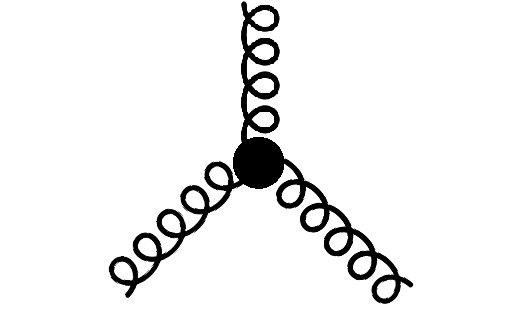
\includegraphics[scale=0.3, valign=c]{figs/diagrams/qcd_action/3gluon_vertex} +
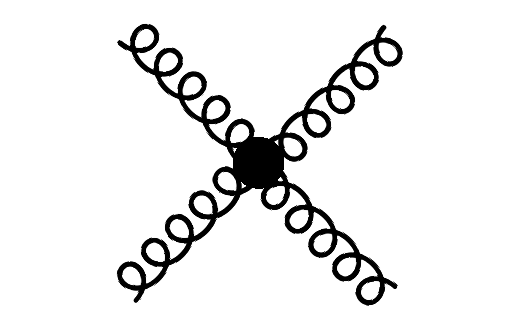
\includegraphics[scale=0.3, valign=c]{figs/diagrams/qcd_action/4gluon_vertex} 
\end{align*}

\caption{Diagrammatical representation of the classical Yang-Mills action featuring the (inverse) gluon propagator and the characteristic cubic and quartic gluon self interactions.}
\label{fig:ym_action}
\end{figure}
\hspace{-0.5em} The gluon field strength tensor $F_{\mu\nu}$ is then constructed as the curvature tensor corresponding to the covariant derivative as usual, i.\,e. 
\begin{equation}
F_{\mu \nu}=\frac{i}{g}\left[D_{\mu}, D_{\nu}\right]=F_{\mu \nu}^{a} T^{a} \quad \text { with } \quad F_{\mu \nu}^{a}=\partial_{\mu} A_{\nu}^{a}-\partial_{\nu} A_{\mu}^{a}+g f^{a b c} A_{\mu}^{b} A_{\nu}^{c},
\end{equation}
and has by construction the desired transformation behavior
\begin{equation}
F_{\mu \nu} \rightarrow F^{\prime}_{\mu \nu}=U F_{\mu \nu}\ U^{\dagger}.
\end{equation}
With this we are finally able to construct the gauge-invariant Yang-Mills action:
\begin{equation}
	S_{\mathrm{YM}}[A] = \frac{1}{2} \int_x \operatorname{Tr}\big[F_{\mu\nu} F_{\mu\nu}\big]\ \overset{(\ref{eqn:normalization})}{=}\  \frac{1}{4} \int_x F_{\mu\nu}^{a} F_{\mu\nu}^{a}.\label{eqn:ym_action}
\end{equation}
Note the factor of $1/2$ coming from the normalization of the generators.
A diagrammatic representation of this action featuring its characteristic properties is presented  in \figref{fig:ym_action}. \\
\noindent Unfortunately we are not finished yet, since the action defined in \eqref{eqn:ym_action} features physically equivalent gauge degrees of freedom, living on the same gauge orbit, i.\,e. all configurations connected via gauge transformations. The next section is denoted to resolve this problem\footnote{This is still not the full solution to the problem, since  we have to be careful with the Gribov ambiguity, i.\,e. that  a gauge fixing submanifold (associated with a specific gauge choice) may not intersect a gauge orbit at all or it may intersect it more than once \cite{Gribov1978}, but we will not focus on this in detail here.} by employing the so-called Faddeev-Popov gauge fixing procedure \cite{FaddeevPopov1967}.
\subsection{Quantization and Gauge Fixing}
As observed before, we have to cope with the fact, that the action (\ref{eqn:ym_action}) features infinitely many redundancies, i.\,e.  physically equivalent field configurations connected via gauge transformations (\ref{eqn:local_gauge_trafo}). 
The general gauge fixing condition can be implemented as
\begin{equation}
\mathcal{F}[A_{\mathrm{gf}} = A^{U(\theta_{\mathrm{gf}})}]=0, \label{eqn:condition}
\end{equation}
with the algebra element $\theta_{\mathrm{gf}}$ being the one that satisfies a certain gauge fixing condition. This corresponds to the explicit choice of one representative per gauge orbit. Concerning this work, we restrict ourselves to the rather general class of linear covariant gauges of the form
\begin{equation}
	\mathcal{F}[A_{\mathrm{gf}}]=l_{\mu}A_{\mu}.
\end{equation}
Here, $l_{\mu}$ can be a differential operator, space-time dependent or a combination thereof \cite{Wink2020}. For a collection of commonly used conventions see below:
\begin{align}
	\mathcal{F}[A_{\mathrm{gf}}]\equiv l_{\mu}A_{\mu},\quad \text{explicitly}\quad \left\{\begin{array}{ll}{\mathcal{F}[A_{\mathrm{gf}}] = \partial_{\mu}A_{\mu},} & {\text{Covariant or Lorenz gauge}} \\ {\mathcal{F}[A_{\mathrm{gf}}] = \partial_iA_i,} & {\text {Coulomb gauge}} \\ {\mathcal{F}[A_{\mathrm{gf}}] = x_{\mu}A_{\mu},} & {\text{Fock-Schwinger gauge}} \\ {\mathcal{F}[A_{\mathrm{gf}}] = n_{\mu}A_{\mu},} & {\text{Axial gauge}} \\ {\mathcal{F}[A_{\mathrm{gf}}]: A_0(x) = A_0^c(\mathbf{x}),} & {\text{Polyakov gauge}}\end{array}\right.
\label{eqn:regulator_limits}
\end{align}
Technically, for a general gauge condition such as in (\ref{eqn:condition}), we can now handle the implementation by splitting the functional integration over the gauge fields into physically inequivalent ($A_{\mathrm{gf}}$) and equivalent, gauge contributions ($\theta$),  
\begin{equation}
\int\mathcal{D} A = \int J\ \mathcal{D}A_{\mathrm{gf}}\ \mathcal{D}\theta, \label{eqn:measure}
\end{equation}
with the Jacobian of the variable transformation $J$ and the so called Haar measure $\mathcal{D}\theta$. Due to the gauge invariance of the action, the integration over the the gauge group factorizes and can be dropped\footnote{Technically, the $\theta$-dependence can be absorbed in $A\rightarrow A^{\theta}$, which directly follows from gauge invariance of the considered quantities. This allows for a cancellation of the respective contributions when computing general observables $\mathcal{O}$. The redundancy is therefore eliminated in the path integral.}. Using the property (\ref{eqn:measure}) and making use of the identity
\begin{equation}
1=\int \mathcal{D} A\ \delta( \mathcal{F})\overset{(\ref{eqn:measure})}{=}\int \mathcal{D} \theta(x)\ \delta\left( \mathcal{F}[A^{\theta}]\right) \operatorname{det}\left(\frac{\delta  \mathcal{F}[A^{\theta}]}{\delta \theta}\right),
\label{eqn:FP_identity}
\end{equation}
where $\delta$ is the functional Dirac delta distribution, we come to the central idea of the Faddeev-Popov trick \cite{FaddeevPopov1967}. The trick is to represent the occurring functional determinant in terms of a Gaussian integral over anti-commuting Grassmann fields, which evaluates for covariant gauges, $\partial_{\mu}A_{\mu}=0$, to 
\begin{equation}
\operatorname{det}\left(\frac{\delta \mathcal{F}^{a}}{\delta \theta^{b}}\right)=\operatorname{det}\left(\frac{1}{g} \partial_{\mu} D_{\mu}^{a b}\right)=\int \mathcal{D} c \mathcal{D} \bar{c}\ \exp \left[\int_{x} \bar{c}^{a} \partial_{\mu} D_{\mu}^{a b} c^{b}\right],
\end{equation}
where we used $\frac{\delta G^{a}}{\delta \theta^{b}}=\frac{\delta G^{a}}{\delta A_{\mu}^{c}} \frac{\delta A_{\mu}^{c}}{\delta \theta^{b}}$ and introduced the covariant derivative in the adjoint representation,
\begin{equation}
D_{\mu}^{a b}=\delta^{a b} \partial_{\mu}-g f^{a b c} A_{\mu}^{c}.
\end{equation}
The fields $c$ and $\bar{c}$ are usually referred to as Faddeev-Popov ghosts and antighosts. They are no physical (= observable) degrees of freedom since they violate the spin statistics theorem. Their sole purpose is to cancel unphysical degrees of freedom and thereby guarantee unitarity \cite{Cyrol2017}. Integrating over the $\delta$-function in (\ref{eqn:FP_identity}) by introducing a Gaussian weighting function of the form 
\begin{equation}
\delta\left[\mathcal{F}[A^{\theta}]\right] \rightarrow \int \mathcal{D}\omega\ \delta\left[\mathcal{F}[A^{\theta}-\omega]\right] \exp \left\{-\frac{1}{2 \xi} \int_{x} \omega^{a} \omega^{a}\right\},
\end{equation}
with arbitrary functions $\omega^{a}(x)$, leads to the explicit appearance of a so called gauge fixing parameter $\xi$ in the theory.
In total, we can now conclude our findings and finally present the expression for the gauge-fixed generating functional of Yang-Mills theory:
\begin{equation}
Z[J]=\int \mathcal{D}A\ \exp \left(S_{\mathrm{YM}}[A]+\int_{x} J_{\mu}^{a} A_{\mu}^{a}\right).
\end{equation}
\paragraph{A Short Introduction to the Superfield Formalism.}

At this point we want to introduce briefly the superfield formalism \cite{QMeS2021, NPgaugeLecture} as a very useful tool to condense our notation in the discussion of the quantization and gauge fixing procedure for general non-Abelian gauge theories. \\
For our concrete example of Yang-Mills theory we collect the field content in a so-called superfield $\Phi = \left(A, c, \bar{c}\right)^T$. The corresponding metric tensor then reads
\begin{equation}
(\gamma)^{a b}=\left(\begin{array}{ccc}
1 & \phantom{-}0 & \phantom{-}0  \\
0 & \phantom{-}0 & \phantom{-}1  \\
0 & -1 & \phantom{-}0  \\
\end{array}\right),
\end{equation}
resulting from  the convention $\Phi_{a}\Phi^{a} = A^2 + 2c\bar{c}$, or in other words the metric $\gamma$ is diagonal in bosonic and symplectic in fermionic subspaces. By convention indices are always raised from the left and lowered from the right, i.\,e.  $\Phi^{a} = \gamma^{ab}\Phi_{b} = \Phi_{b}\gamma^{ab} = \left(A, c, \bar{c}\right)$ which directly implies the following identities:
\begin{align}
	\gamma_{a}^{\phantom{a}b} &= \gamma^{bc}\gamma_{ac} = \delta^{b}_{\phantom{c}a} \\
	\gamma^{a}_{\phantom{a}b} &= \gamma^{ca}\gamma_{bc} = (-1)^{ab}\delta^{a}_{\phantom{c}b},
\end{align}
where 
\begin{equation}
\begin{aligned}
	(-1)^{ab} = \left\{\begin{array}{ll}{-1} & {\text { if } a\ \text{and}\ b \text { fermionic, } } \\ {\phantom{-}1} & {\text { otherwise. }} 
	\end{array}\right.
\end{aligned}
\end{equation}
This condensed notation allows us to write all relevant functionals and equations including sets of multiple fields of different kinds  in a short and concise way.\\
Applying these conventions to our equations leaves us with the following expression for the gauge fixed generating functional for Yang-Mills theory,
\begin{equation}
Z\left[J\right]=\int \dd \Phi\ \exp\left(-S_{\mathrm{YM}}[\Phi]+J_{\Phi}\cdot \Phi\right),
\end{equation}
with the Yang-Mills superfield $\Phi$ as above, and the corresponding supercurrent, 
\begin{equation}
\begin{aligned}
J_{\Phi} &= (J_A, J_c, J_{\bar{c}}).
\end{aligned}
\end{equation}
The gauge-fixed action $S_A$ now features the  gauge fixing and ghost terms, as derived before, 
\begin{equation}
S_{\mathrm{YM}}[\Phi]=\underbrace{\frac{1}{4} \int_{x} F_{\mu \nu}^{a} F_{\mu \nu}^{a}}_{S_{\mathrm{gauge}}}+\underbrace{\frac{1}{2 \xi} \int_{x}\left(\partial_{\mu} A_{\mu}^{a}\right)^{2}}_{S_{\mathrm{gf}}}-\underbrace{\int_{x} \bar{c}^{a} \partial_{\mu} D_{\mu}^{a b} c^{b}}_{S_{\mathrm{gh}}}.
\end{equation}
The explicit choice of the gauge fixing parameter $\xi$ can simplify computations a lot. A common choice for perturbative calculations is $\xi=1$, which is known as \textit{Feynman gauge}. We decided to work in \textit{Landau gauge} corresponding to the choice $\xi=0$, which has to be understood as taking the limit $\xi\rightarrow 0$ after deriving the explicit expressions. For most applications of functional methods Landau gauge is the standard way to go, since it allows for a complete decoupling of the longitudinal and transversal parts  of the respective equations. This will be made clear in the subsequent discussion of our calculations in \chapref{chap:results}.
 

\section{From Yang-Mills to QCD}\label{sec:ym_to_qcd}
Up to now, we only focused on the pure gauge part of the theory. To arrive at the final expression for the full QCD action, we need to introduce quarks. The corresponding action for free quarks is given by the usual Dirac action for fermions, the minimal coupling between the quarks and gluons is again realized by promoting the partial derivatives to covariant ones, cf. (\ref{eqn:covariant_derivative}). This yields
\begin{equation}
S_{\mathrm{Dirac}}[A,\bar{\psi},\psi]=\int_x \bar{\psi}(i\slashed{D} + m_{\psi}) \psi,
\end{equation}
with the spin-$\frac{1}{2}$ spinor fields $\psi = (\psi_1, \dots, \psi_{N_f})$ for $N_f$ quark flavors carrying a Dirac index, gauge group indices in the fundamental representation and flavor indices. The respective current quark masses $m_{\psi}$ are diagonal in flavor space as well as the covariant derivative. As usual, the Feynman slash notation implies contractions with gamma matrices\footnote{In the discussion of Dirac fermions, the gamma matrices $\left\{\gamma_0, \gamma_1, \gamma_2, \gamma_3\right\}$ are a set of complex valued matrices that constitute an irreducible representation of the Clifford algebra  defined by the anticommutation relation $\left\{\gamma_{\mu}, \gamma_{\nu}\right\}= 2g_{\mu\nu} \mathbbm{1}_{d_{\gamma}\times d_{\gamma}}$, with $d_{\gamma} = 2^{\left[\sfrac{d}{2}\right]}$\ \cite{PeskinSchroeder1995}.\\}, i.\,e. $\slashed{D} = \gamma^{\mu}D_{\mu}$.
 Concerning notation, the spinor fields $\psi$ represent the (up to) six quark flavors 
  \begin{equation}
  \begin{aligned}
 	\psi \equiv q &= \left(\text{up}, \text{down}, \text{strange}, \text{charm}, \text{top}, \text{bottom}\right), \\
 	&= \left(u, d, s, c, t, b\right).
 	 \end{aligned}
 \end{equation}
For most applications one usually works in a 2-flavor setting\footnote{Often also 2+1-flavor settings, involving the \enquote{heavy} strange quark are considered.}, ignoring the heavier quarks, since their mass hierarchy is very large, i.\,e. the masses rise quickly from flavor to flavor, with the exception of the first generation involving the up and down quark. As we are working in the low-energy, infrared regime of QCD, the 2-flavor approximation is well justified since the heavier quarks only become relevant at scales far above the QCD phase transition scale at about $T\approx 155$\ MeV for vanishing chemical potential. \\
After having discussed all relevant components, we are now ready to present the generating functional for the fully quantized theory of QCD, involving the pure gauge Yang-Mills part as derived before and the quarks, represented as Grassmann fields, due to their fermionic nature:
\begin{equation}
Z\left[J\right]=\int \mathcal{D}\Phi\ \exp\left(-S_{\mathrm{QCD}}[\Phi]+J_{\Phi}\cdot \Phi\right),
\label{eqn:Z_QCD}
\end{equation}
with the QCD superfield $\Phi$, and supercurrent $J$, 
\begin{equation}
\begin{aligned}
\Phi &= (A, c, \bar{c}, q, \bar{q})\\
J_{\Phi} &= (J_A, J_c, J_{\bar{c}}, J_{q}, J_{\bar{q}}).
\end{aligned}
\end{equation}
The corresponding gauge-fixed action $S_{\mathrm{QCD}}[\Phi]$ in (\ref{eqn:Z_QCD}) for a general covariant  gauge is given by
\begin{equation}
S_{\mathrm{QCD}}[\Phi]= \int_{x}\left\{\frac{1}{4}F_{\mu \nu}^{a} F_{\mu \nu}^{a}+\frac{1}{2 \xi}\left(\partial_{\mu} A_{\mu}^{a}\right)^{2}-\bar{c}^{a} \partial_{\mu} D_{\mu}^{a b} c^{b}+\bar{q}\left(i\slashed{D}+m_{q}\right) q\right\}.
\label{eqn:S_QCD}
\end{equation}
Again, we provide a diagrammatical representation of the action (\ref{eqn:S_QCD}) in \figref{fig:S_QCD}. To conclude our discussion of the basic concepts of QCD, we can now explicitly derive and have a look at the functional relations relevant for the remainder of the work in the following section.
\begin{figure}[t]
\centering
\begin{align*}
\hspace{-1.5em}S_{\mathrm{QCD}}\left[\Phi\right] =
(
\includegraphics[scale=0.16, valign=c]{figs/diagrams/qcd_action/gluon_propagator})^{-1} +
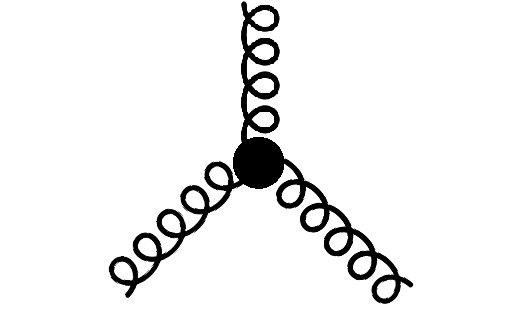
\includegraphics[scale=0.16, valign=c]{figs/diagrams/qcd_action/3gluon_vertex} +
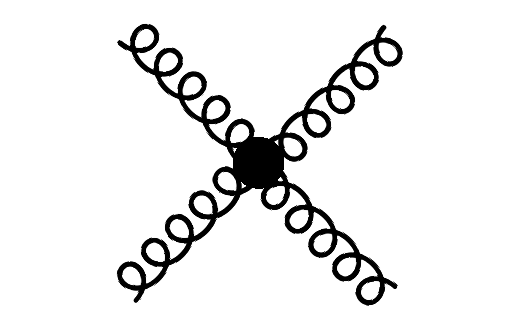
\includegraphics[scale=0.16, valign=c]{figs/diagrams/qcd_action/4gluon_vertex} +
(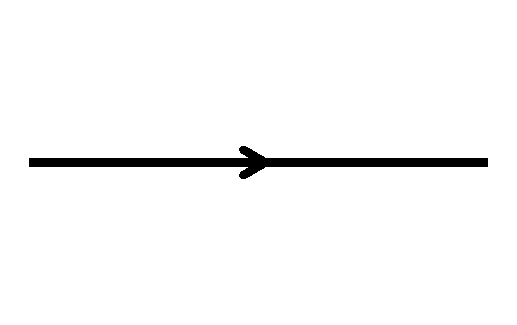
\includegraphics[scale=0.16, valign=c]{figs/diagrams/qcd_action/quark_propagator})^{-1} +
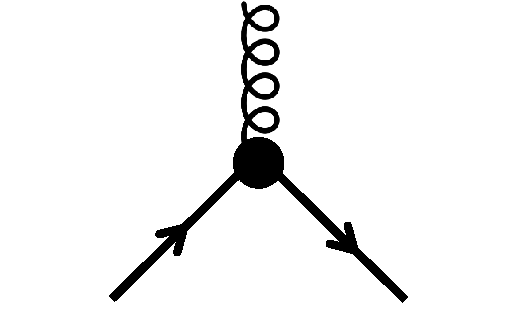
\includegraphics[scale=0.16, valign=c]{figs/diagrams/qcd_action/quark_gluon_vertex} +
(
\includegraphics[scale=0.16, valign=c]{figs/diagrams/qcd_action/ghost_propagator})^{-1} +
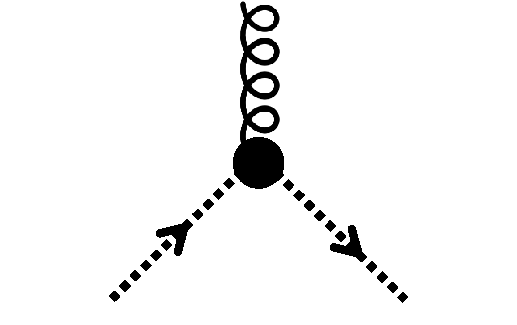
\includegraphics[scale=0.16, valign=c]{figs/diagrams/qcd_action/ghost_gluon_vertex}
\end{align*}

\caption{Diagrammatical representation of the QCD action. Compared to the Yang-Mills case we find in addition the (inverse) quark and ghost propagators and the respective interaction vertices with the gluons.}
\label{fig:S_QCD}
\end{figure}

\section{Dyson-Schwinger Equations for Yang-Mills and QCD}\label{sec:ym_qcd_dse}
Combining the results introduced in the two previous chapters, we now want to finally discuss, at least schematically, the functional relations that will be of great importance for the remainder of this work.\\
The quark propagator DSE\footnote{The addition \enquote{propagator} will be left out occasionally throughout this thesis, using \enquote{quark (gluon/ghost) DSE} synonymously to \enquote{quark (gluon/ghost) propagator DSE} if not explicitly stated otherwise.} can be derived from the master DSE (\ref{eqn:DSE}), this time using the QCD action (\ref{eqn:S_QCD}), the same way as explained for the scalar case earlier. Schematically it reads
\begin{equation}
\Gamma_{q \bar{q}}^{(2)}=S_{q \bar{q}}^{(2)}-S_{q \bar{q} A}^{(3)} \cdot G_{q} \cdot \Gamma_{q \bar{q} A}^{(3)} \cdot G_{A},\label{eqn:quark_DSE}
\end{equation}
with the quark and gluon propagators $G_q$ and $G_A$, and the classical and full quark-gluon vertices $S_{q \bar{q} A}^{(3)}$ and $\Gamma_{q \bar{q} A}^{(3)}$. As before, a diagrammatical representation of this equation is presented in \figref{fig:quarkDSE} at the beginning of the next page. It relates the full (inverse) two-point function to the bare propagator plus higher loop order diagrams, in our case the one-loop quark self energy $\Sigma_q$.\\
 We will postpone the discussion about regularization and renormalization of the diagrams to the main part of this work, where we will guide the reader step by step through the entire process of accessing the spectral functions from the DSE. \\
 The attentive reader might notice, that the quark DSE also needs the gluon propagator and the quark-gluon vertex as non-trivial external input. For the gluon propagator $G_A$, there has been a lot of progress in recent years, mainly with the help of reconstruction techniques, cf. \cite{Cyrol2017, CyrolMitterPawlowskiStrodthoff2017, CyrolPawlowskiRothkopWink2018}, and also just recently via the spectral approach used in this work. Note that the results we are stating here are partially not yet published. Details of the chosen external input will again be discussed in the respective chapter. 
The full vertex could in principle also be included via its spectral representation in this setting, but for a first attempt, it is approximated as the classical quark-gluon vertex, i.\,e. $\Gamma^{(3)} = S^{(3)}$.\\
To conclude our discussion, we will present the respective equations for the Yang-Mills sector in the following. The gluon DSE schematically reads
\begin{equation}
\Gamma_{A A}^{(2)}=S_{A A}^{(2)}-\frac{1}{2} S_{A A A}^{(3)} \cdot G_{A} \cdot \Gamma_{A A A}^{(3)} \cdot G_{A}+ \frac{1}{2}S_{c \bar{c} A}^{(3)} \cdot G_{c} \cdot \Gamma_{c \bar{c} A}^{(3)} \cdot G_{c}+ \text{higher loops}.\label{eqn:gluon_DSE}
\end{equation}
It inherits the same problem as the quark DSE, since it depends on the external input of the ghost propagator and the respective vertex, and vice versa for the ghost DSE. Therefore we have to deal with a dynamically coupled system of equations. This is already the main difference to the scalar case discussed in \chapref{chap:methods}, i.\,e. the appearance of a second field complicates the structure of the equations already a lot. Note also, that for the gluon DSE we only presented the expression up to one loop for feasibility. Solving this system for the Yang-Mills case only was the purpose of the work put forward in \cite{Horak2019}.\\ 
Although it is not directly important for our explicit calculations, for the sake of completeness, we also give the expression for the ghost propagator DSE,
\begin{equation}
\Gamma_{c \bar{c}}^{(2)}=S_{c \bar{c}}^{(2)}-S_{c \bar{c} A}^{(3)} \cdot G_{c} \cdot \Gamma_{c \bar{c} A}^{(3)} \cdot G_{A},\label{eqn:ghost_DSE}
\end{equation}
which looks very similar to the quark DSE. Here, the only non-trivial contribution is given by the ghost self-energy $\Sigma_c$. In an analogous analysis of the ghost DSE as compared to our work, spectral functions could be successfully computed. The results have just been published recently by group members and collaborators, cf. \cite{HorakPapavassiliouPawlowskiWink2021}. In analogy to the quark DSE, we present the respective diagrammatical representations of the gluon and ghost DSEs in \figref{fig:YM_DSEs}.\\

\begin{figure}[t]
\centering
\begin{align*}
\bigg(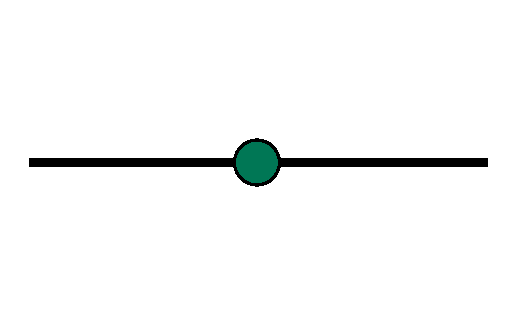
\includegraphics[scale=0.4, valign=c]{figs/diagrams/quarkDSE/full_quark_propagator}\bigg)^{-1} = 
\bigg(
\includegraphics[scale=0.4, valign=c]{figs/diagrams/quarkDSE/bare_quark_propagator.pdf}\bigg)^{-1} - 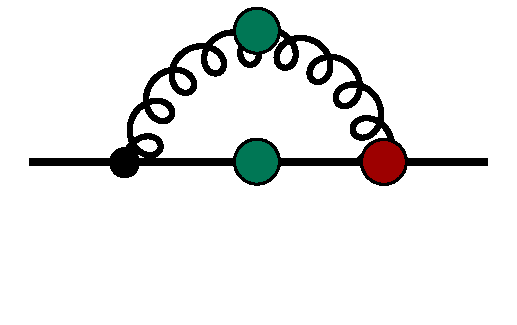
\includegraphics[scale=0.4, valign=c]{figs/diagrams/quarkDSE/quark_self_energy}
\end{align*}

\caption{Diagrammatic representation of the quark propagator DSE, often referred to as the quark gap equation. The non-trivial contribution is given by the one-loop quark self energy $\Sigma_q$.}
\label{fig:quarkDSE}
\end{figure}
\newpage
\begin{figure}[H]
\centering
\begin{align*}
\bigg(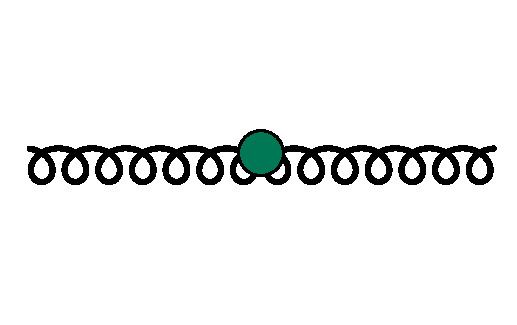
\includegraphics[scale=0.3, valign=c]{figs/diagrams/gluonDSE/full_gluon_propagator}\bigg)^{-1} &= 
\bigg(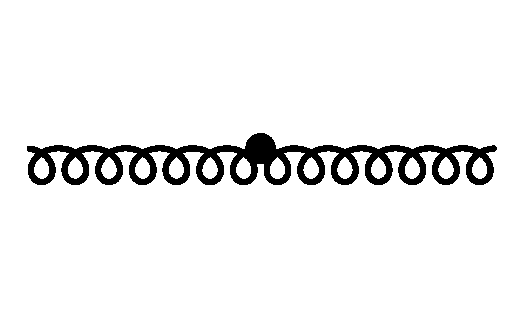
\includegraphics[scale=0.3, valign=c]{figs/diagrams/gluonDSE/bare_gluon_propagator.pdf}\bigg)^{-1}\ - \frac{1}{2}\ 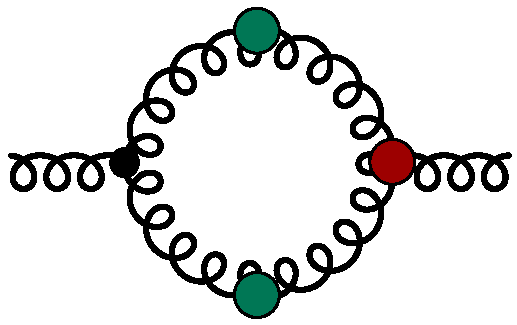
\includegraphics[scale=0.3, valign=c]{figs/diagrams/gluonDSE/gluon_polarization}\ +\ \frac{1}{2}\ 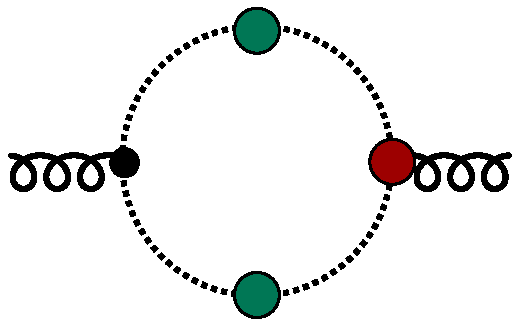
\includegraphics[scale=0.3, valign=c]{figs/diagrams/gluonDSE/ghost_polarization}  \\[0.8em]
\bigg(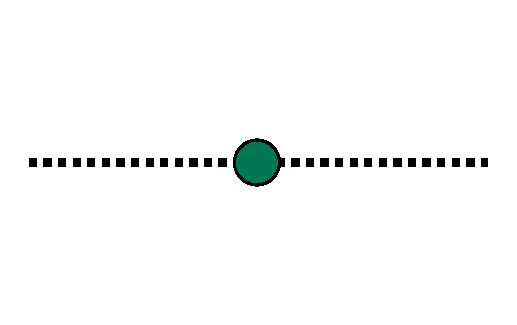
\includegraphics[scale=0.3, valign=c]{figs/diagrams/ghostDSE/full_ghost_propagator}\bigg)^{-1} &= 
\bigg(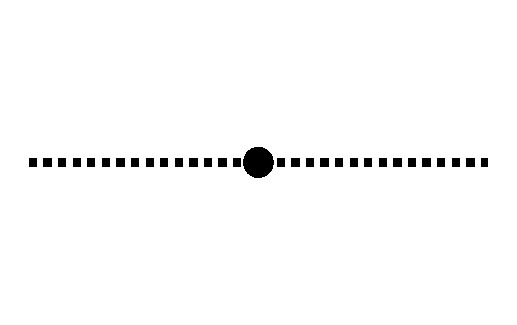
\includegraphics[scale=0.3, valign=c]{figs/diagrams/ghostDSE/bare_ghost_propagator.pdf}\bigg)^{-1}\hspace{0.625em} -\hspace{0.625em}   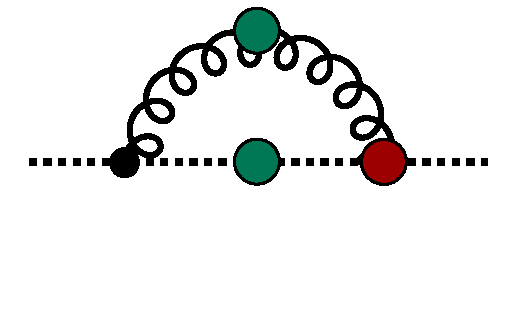
\includegraphics[scale=0.3, valign=c]{figs/diagrams/ghostDSE/ghost_self_energy} \\[0.8em]
\bigg(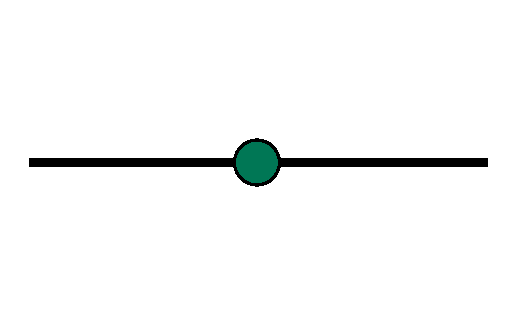
\includegraphics[scale=0.3, valign=c]{figs/diagrams/quarkDSE/full_quark_propagator}\bigg)^{-1} &= 
\bigg(
\includegraphics[scale=0.3, valign=c]{figs/diagrams/quarkDSE/bare_quark_propagator.pdf}\bigg)^{-1}\hspace{0.625em} -\hspace{0.625em} 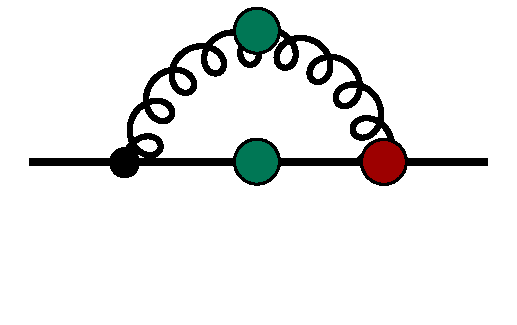
\includegraphics[scale=0.3, valign=c]{figs/diagrams/quarkDSE/quark_self_energy}
\end{align*}

\caption{Diagrammatical representation of the gluon and ghost propagator DSEs according to equations (\ref{eqn:gluon_DSE}) and (\ref{eqn:ghost_DSE}). The gluon DSE is truncated at one loop.}
\label{fig:YM_DSEs}
\end{figure}


	\chapter{Quark Spectral Functions in QCD}\label{chap:results}
This chapter summarizes the main part of our work. The goal  is to find a K\"all\'{e}n-Lehmann spectral representation of the quark propagator by iteratively solving the corresponding Dyson-Schwinger equation. Employing the KL spectral representation of the quark and gluon propagators allows for a perturbative treatment of the occurring loop diagram at the expense of additional spectral integrals for every propagator, and basically also for every higher $n$-point function\footnote{Whereas axiomatic approaches to QFT predict their existence in general, there has not yet been a lot of work on spectral representations for higher order $n$-point functions. } involved in the computation. The spectral renormalization scheme put forward in \cite{Horak2019,Wink2020,HorakPawlowskiWink2020} provides a well suited  framework for a practical numerical implementation of our problem while maintaining all underlying symmetries of the theory at hand.\\
 The first part of this chapter provides a detailed introduction to the general methodology of the spectral renormalization scheme. The aim  is to guide the reader through the most important steps of the conducted calculations using the concrete example of the quark DSE, focusing on the conceptually most important steps. For technical details concerning the calculations, we refer the interested reader to \appref{chap:appendixA}.
In the second part we focus on the iterative solution of the quark DSE and comment on the numerical implementation. Subsequently, we present and discuss our results.

\section{Methodology of the Spectral Renormalization Scheme}
As motivated in the introduction of this chapter, using the KL spectral representation of the propagators in functional equations, such as in our case the quark DSE displayed in \figref{fig:quarkDSE}, allows for a perturbative treatment of the occurring loop momentum integrals appearing naturally in the respective  diagrams, here on the right-hand side of the equation. This allows us to get analytical access to the Euclidean momentum structure of the relevant diagram(s) and therefore of the whole equation. \\
Maybe the most important advantage of the possibility to treat the occurring diagrams perturbatively, is that this allows for the application of well established  renormalization techniques, in order to cancel possible UV divergencies. In our specific case, the loop momentum integrations are rendered finite using the manifestly gauge-invariant dimensional regularization scheme, cf. \cite{Leibbrandt1975, PeskinSchroeder1995}, in combination with a BPHZ-type subtraction scheme for the spectral integrands, cf.  \cite{BogolyubovParasiuk1954,Hepp1966,Zimmermann1969}.\\
 The subsequently discussed spectral renormalization scheme put forward in  \cite{Horak2019,Wink2020,HorakPawlowskiWink2020}, consists of a twofold treatment of the respective loop momentum integrals, leading to finite expressions for the spectral integrands, that can be used as an input for numerical applications, that are usually unavoidable in non-perturbative calculations.  For a schematic  overview of the applied regularization procedure, cf. \figref{fig:spectral_renormalization}.\\
 \begin{figure}[t]
\centering
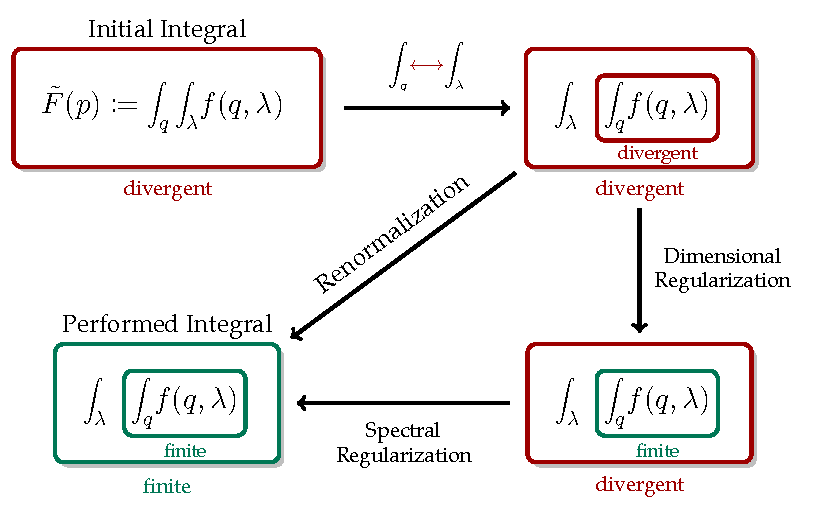
\includegraphics[width=0.8\textwidth]{figs/tikz/spectral_renormalization}
\caption[Applied regularization procedure.]{Applied regularization procedure. $f$ is some arbitrary divergent integrand. The two upper boxes have to be understood as finite by dimensional regularization but divergent in the limit $\varepsilon\rightarrow 0$. The first step consists of evaluating the momentum integral analytically using dimensional regularization \cite{Leibbrandt1975} before renormalizing the spectral integrands subsequently according to a BPHZ-renormalization scheme \cite{BogolyubovParasiuk1954, Hepp1966, Zimmermann1969}.}\label{fig:spectral_renormalization}
\end{figure}
\noindent
We will motivate the application of this scheme at the concrete example of our calculation of the quark self energy diagram, given by
\begin{align}
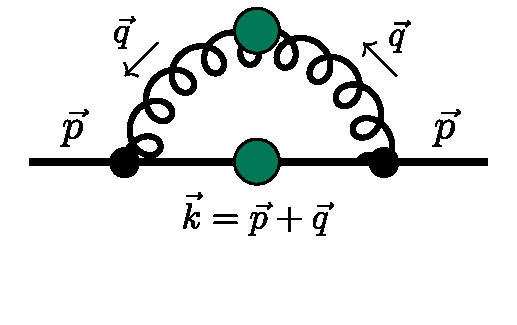
\includegraphics[scale=0.45, valign=c, trim = 0 6em 0 0]{figs/diagrams/quark_self_energy_classical} := \Sigma_q
(p) &= (-ig)^2 \delta^{ab}C_f \int_q\ \Pi^{\mu\nu}_{\perp}(q) G_A(q)\gamma_{\mu}G_q(p+q)\gamma_{\nu},
\end{align}
employing the Feynman rules for QCD in the Landau gauge. Note, that throughout this work, we will approximate the full quark-gluon vertex by its classical, bare counterpart:
 \begin{equation}
 	\Gamma^{(3)}_{q\bar{q}A} \equiv S^{(3)}_{q\bar{q}A},
 \end{equation}
leaving us with one spectral integral for the gluon and one for the quark propagator, respectively. The gluon and quark propagators are parametrized as 
\begin{align}
\left[G_{A}\right]_{\mu \nu}^{a b}&=\delta^{a b}\ \Pi_{\mu \nu}^{\perp}(p)\ G_{A}(p) + \frac{1}{\xi} \delta^{a b}\ \Pi_{\mu \nu}^{\|}(p)\ p^{2},\\
\left[G_{q}\right]^{a b} &= \delta^{ab}G_q(p),
\end{align}
with the longitudinal and transversal projectors defined as 
\begin{align}
\Pi_{\|}^{\mu \nu}(p)&=\frac{p^{\mu} p^{\nu}}{p^{2}},\\
\Pi_{\perp}^{\mu \nu}(p)&= \delta^{\mu\nu} - \Pi_{\|}^{\mu\nu}(p). \label{eqn:transversal_projector}
\end{align}
The advantage of working in Landau gauge, hence employing $\xi\rightarrow 0$, is, that it  allows for a closure of the transversal sector and the longitudinal components of the presented parameterization of the gluon propagator do not explicitly enter our calculation, cf. \cite{CyrolFisterMitterPawlowskiStrodthoff2016}. The quark DSE is projected onto $G_q$ via the application of a color trace, i.\,e. 
\begin{equation}
\left[\Gamma_{q}^{(2)}\right]^{a b}\quad \longrightarrow\quad \delta_{a b} \left[\Gamma_{q}^{(2)}\right]^{a b}.
\end{equation}
For the parts of the propagators, that are independent of the Lorentz and color structure, we insert the spectral representations
\begin{align}
G_{A}(q)&= \int_{\lambda_1}\ \frac{\lambda_1\rho_A(\lambda_1)}{q^{2}+\lambda_1^{2}},\label{eqn:GluonSpec}\\[1em]
G_q(p+q) &= -i(\slashed{p}+\slashed{q})\cdot G_{q}^{D}(p+q)+G_{q}^M(p+q)\nonumber \\
&= (\slashed{p}+\slashed{q}) \int_{\lambda_2}\ \frac{\lambda_2\rho_{q}^D(\lambda_2)}{(p+q)^{2}+\lambda_2^2}+ \int_{\lambda_2}\ \frac{\lambda_2\rho_{q}^M(\lambda_2)}{(p+q)^{2}+\lambda_2^2},\label{eqn:QuarkSpecFunc}
\end{align}
with the conventions for the spectral integrations given by
\begin{equation}
	\int_{\lambda_i} = \int_0^{\infty} \frac{\dd\lambda_i}{\pi} \qquad \text{and} \qquad \int\limits_{\left\{\lambda_i,\lambda_j\right\}} = \int_0^{\infty} \frac{\dd\lambda_i}{\pi}\frac{\dd\lambda_j}{\pi}.	 
\end{equation}
The detailed discussion on the Dirac structure of the quark propagator is moved to \appref{chap:appendixB}. For the sake of completeness, the full expression for the quark propagator in terms of the two dressing functions $Z_q(p)$ and $M_q(p)$ is given in the following:
\begin{equation}
	G_q(p) =  -i\slashed{p} \left(\frac{Z_q(p)}{p^2 + M_q^2(p)}\right) +  \left(\frac{Z_q(p)M_q(p)}{p^2 + M_q^2(p)}\right)
\end{equation}
The splitting of the quark propagator into two distinct parts, referred to as Dirac vector ($\sim i\slashed{p}$) and Dirac scalar ($\sim\mathbb{1}$) part, respectively, allows for a separation of the calculation of the diagram according to
\begin{equation}
	\Sigma_q(p) =\slashed{p}\cdot\Sigma_{q}^D(p) + \Sigma_{q}^M(p),
\end{equation}
leading us to two independent integral equations, i.\,e.
\begin{align}
\Sigma_{q}^D(p) &= (-ig)^2\delta^{ab}C_f\int\limits_{\left\{\lambda_1,\lambda_2\right\}}\lambda_1\lambda_2\rho_A(\lambda_1)\rho_q^D(\lambda_2)\cdot I_q^D\left(p, \lambda_1, \lambda_2,x\right),\\
\Sigma_{q}^M(p) &= (-ig)^2\delta^{ab}C_f\int\limits_{\left\{\lambda_1,\lambda_2\right\}}\lambda_1\lambda_2\rho_A(\lambda_1)\rho_q^M(\lambda_2)\cdot I_q^M\left(p, \lambda_1, \lambda_2,x\right).
\end{align}
As already mentioned before, we will \textit{not} display the full, lengthy analytic expressions for the integrands here, but in \appref{chap:appendixA}. \\
Note, that we already implicitly performed the first non-trivial step of the calculation, which consists of swapping the integration order $q\leftrightarrow\{\lambda_1,\lambda_2\}$, corresponding to the step from upper left to the upper right box in \figref{fig:spectral_renormalization}. This is only valid for the case, that both integrations are finite by themselves according to Fubinis theorem. At this point, the finiteness of both integrations is explicitly assumed.\\
By naive power counting, we directly see that the considered diagram is superficially divergent. This requires us to set up a suitable regularization procedure for the integrands in order to proceed with the calculation. For the first part of the calculation, the loop momentum integration is rendered finite by means of dimensional regularization, hence the integrands are evaluated for $d= 4 -2\varepsilon$ and expanded up to lowest order in the limit $\varepsilon\rightarrow 0$. This isolates the divergence of the diagram in the 1/$\varepsilon$-term, which is discarded, as usual. The applicability of dimensional regularization comes with many advantages since it respects all space-time, internal and gauge symmetries of the theory at hand, in contrast to other regularization schemes, that require for example the introduction of explicit cutoffs.  \\
However, the remaining spectral integrands are a priori still \textit{not} finite simply by discarding the 1/$\varepsilon$-term,  which is a remnant of initially swapping the integration order. We are left with finite spectral integrands for $\varepsilon >0$, that in general need to be computed numerically. For numerical performance it is helpful to perform the spectral integrations at $\varepsilon=0$. The same is true for the access to the analytical momentum structure needed to extract the Minkowski properties. It is therefore required to set up a suitable renormalization procedure for the integrands in the limit $\varepsilon\rightarrow 0$. 
 This problem can be resolved by extending the standard dimensional regularization procedure by introducing additional counterterms on the level of the classical action, that cancel the leading and subleading divergent contributions to the spectral integrands.\\ Technically this is implemented by subtracting a Taylor expansion in all momenta around the renormalization group scale $\mu$\footnote{The integrand already depends inherently on the RG scale $\mu$ due to dimensional regularization. \\}, which modifies the UV behavior of the integrand to drop off faster\footnote{We have to cope with the fact, that  the underlying BPHZ-scheme in general does not preserve all symmetries of a given theory and in particular breaks gauge symmetry, but this is also true for other subtraction schemes that introduce explicit counterterms, while leading to  gauge-consistent results.}.  This procedure is called spectral BPHZ-renormalization, cf. \cite{HorakPawlowskiWink2020, BogolyubovParasiuk1954,Hepp1966,Zimmermann1969}. 
 For a schematic overview, cf. \figref{fig:BPHZ}. We visualized the explicit effects of this procedure on the respective integrands in the appendix in \figref{fig:BPHZ_demonstration}.
 The introduced counterterms therefore explicitly contribute to the mass renormalization $M_q(p)$ as well as to the wave function renormalization $Z_q(p)$, characterizing the momentum dependence of the quark propagator, cf. \appref{chap:appendixB} for a detailed discussion. The counterterms consistently remove the divergent parts of the integrands and we explicitly checked for UV-finiteness of all integrations. This finally allows us to solve the spectral integrals numerically after successfully performing the limit $\varepsilon\rightarrow 0$ beforehand.
 \begin{figure}[t]
	\centering
	\begin{align*}
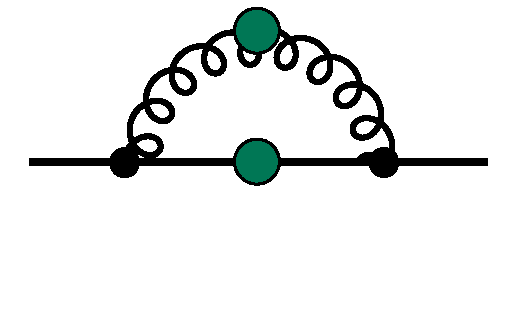
\includegraphics[scale=0.28, valign=c]{figs/diagrams/bphz/quark_self_energy_classical} \longrightarrow 
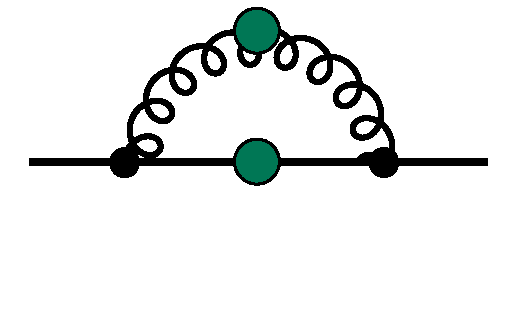
\includegraphics[scale=0.28, valign=c]{figs/diagrams/bphz/quark_self_energy_classical} - \eval{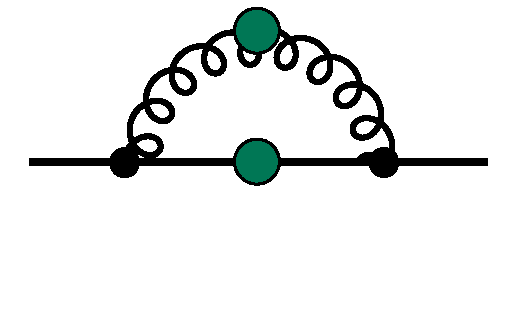
\includegraphics[scale=0.28, valign=c]{figs/diagrams/bphz/quark_self_energy_classical}}_{p=\mu} -\ \frac{(p^2-\mu^2)}{2\mu}\left[\partial_{p}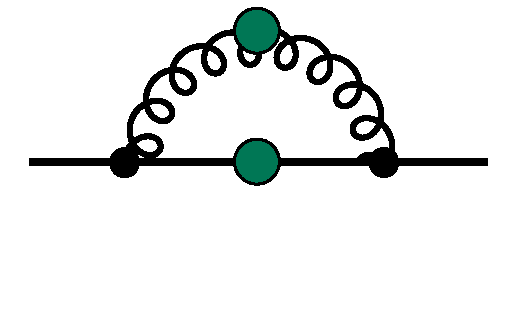
\includegraphics[scale=0.28, valign=c]{figs/diagrams/bphz/quark_self_energy_classical}\right]_{p=\mu}
\end{align*}

	\caption[Schematic spectral BPHZ-renormalization procedure at the example of the quark self energy diagram.]{Schematic spectral BPHZ-renormalization procedure at the example of the quark self energy diagram. The diagram is subtracted by the first two terms of its own Taylor expansion around the RG scale $\mu$ in order to cancel quadratic and logarithmic divergences of the spectral integrands. For a demonstration of the actual effects of the subtraction scheme on the spectral integrands, we refer to \figref{fig:BPHZ_demonstration} in the appendix.} 
	\label{fig:BPHZ}
\end{figure}
Note, that although this might seem like two separate regularization procedures, the above subtraction scheme really just corresponds to the correct application of dimensional regularization. Technically this corresponds to evaluating the integrals at some point $\alpha$ in the complex exponent plane, where the integration is finite. Afterwards all terms are expanded in a Laurent series around $\alpha=d$, and subtracting the first term of this series removes all singularities of this construction by employing finite renormalization conditions. This naturally discards the divergent parts of the spectral integrals, as they depend on the dimension $d$ \cite{Leibbrandt1975, Horak2019}.
In a last step, the (now appropriately regularized) Euclidean expressions can be analytically continued to the real momentum axis according to 
\begin{equation}
	I_q^{(D/M)}\left(\omega, \lambda_1, \lambda_2\right) := I_q^{(D/M)}\left(-i(\omega + i0^+)\right).
\end{equation}
This needs to be done, since the spectral functions are obtained from the retarded propagator. For a visualization, cf. \figref{fig:continuation}.

\section{Iterative Procedure}
With the finite Euclidean and real-time expressions for the spectral integrands $I_q^{(D/M)}(p/\omega)$ at hand, the DSE is now solved iteratively, by performing the spectral integrations and extracting the spectral functions $\rho_q^{(D/M)}$ from the respective parts of the retarded propagator via \eqref{eqn:specfunc_relation}, or to be more precise via \eqref{eqn:correct_relation}. The updated result for the quark spectral functions are then fed back into the computation of the diagram until convergence of the result (by eyesight) is observed. A detailed overview of our numerical workflow is depicted in \figref{fig:numerics}. For explicit details concerning the numerical implementation, we refer to \appref{chap:appendixC}.\\
\begin{figure}[t]
	%\centering
	\hspace{-4.5em}
	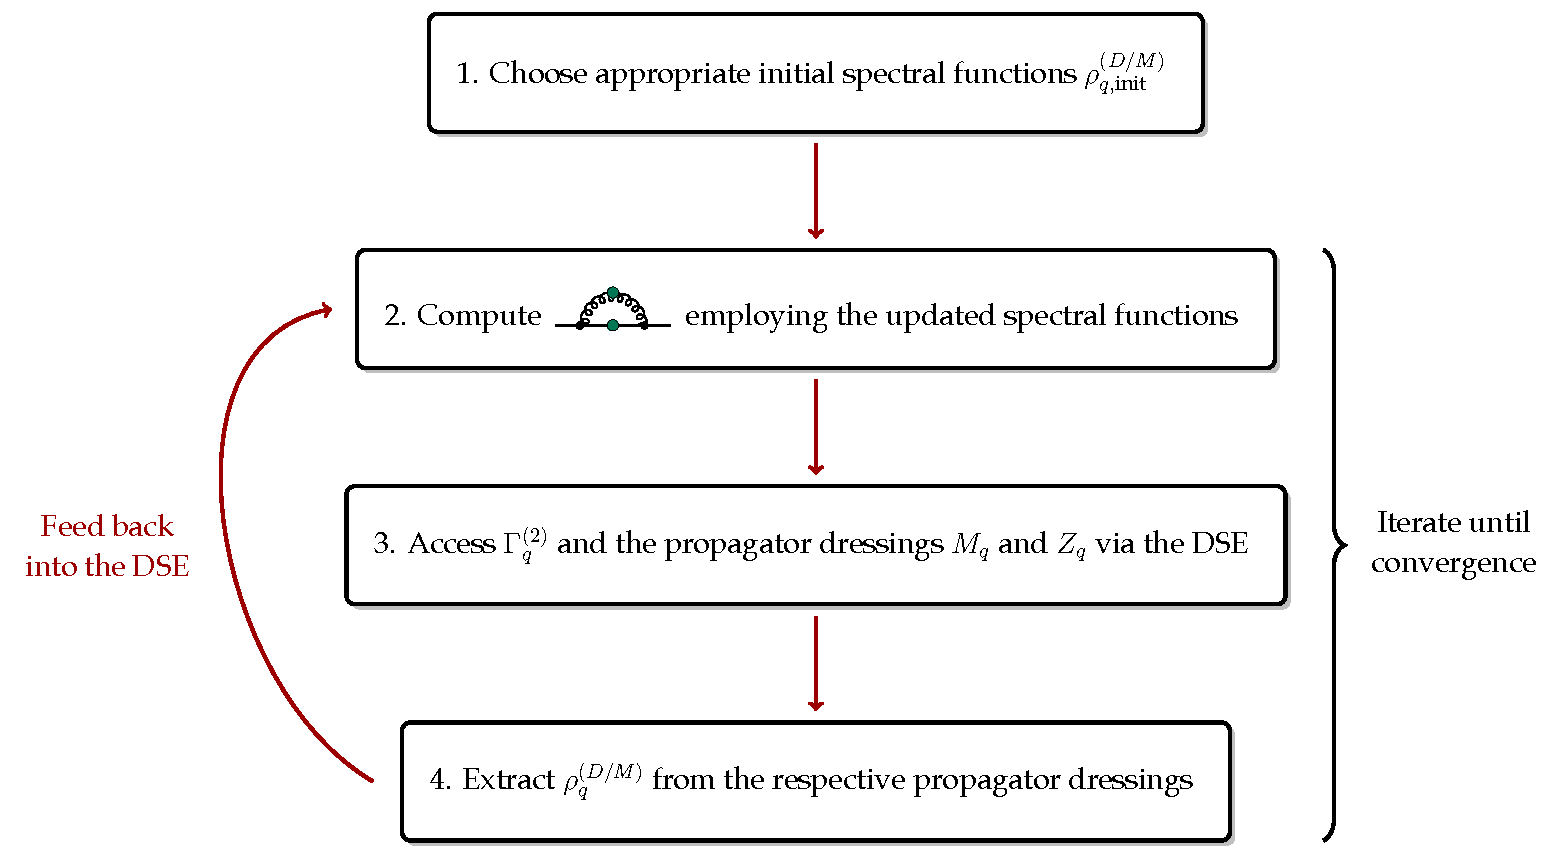
\includegraphics[width = 1.2\textwidth]{figs/tikz/iterative_computation}
	\caption{Iterative procedure to extract the spectral function from the DSE.} 
	\label{fig:numerics}
\end{figure}
Before starting the iterative procedure, appropriate initial \enquote{guesses} for both quark spectral functions $\rho_q^D(\lambda_2)$ and $\rho_q^M(\lambda_2)$ have to be made. A well motivated guess for the quark spectral functions is to employ quasi-classical spectral functions, reproducing  the classical, perturbative quark propagator. They are simply given by (massive) delta distributions:
	\begin{align}
		\rho_{q,\mathrm{init}}^D(\lambda) &= 2\pi i\ \frac{\delta(\lambda-m_q)}{2\lambda}\\
		\rho_{q,\mathrm{init}}^M(\lambda) &= 2\pi m_q\ \frac{\delta(\lambda-m_q)}{2\lambda}.
	\end{align}
The gluon input is considered as \enquote{static} in our computation. The gluon spectral function $\rho_A$ of our choice is given analytically and does not need to be updated after every iteration step. For this concrete example, $\rho_A$ was obtained in \cite{CyrolPawlowskiRothkopWink2018} by reconstruction from numerical data for the Euclidean gluon propagator. This specific result for the gluon spectral function respects the so called \textit{decoupling} (or \textit{massive}) solution for the gluon propagator in the infrared \cite{vonSmekalAlkoferHauck1997}. In future studies, this might be adapted to solutions respecting the known \textit{scaling scenario} \cite{LercheVonSmekal2002}, which has been found to provide a dynamical generation of a mass gap for both the gluon and the ghost propagators, but is in general more complicated due to the non-trivial scaling exponent $\kappa$ with $\frac{1}{2}<\kappa < 1$, slighty modifying the explicit IR behavior .
For a visualization of the chosen gluon spectral function and the corresponding gluon propagator, cf. \figref{fig:gluon_specfunc_and_prop}.
\begin{figure}[t]
\hfill
	\centering
	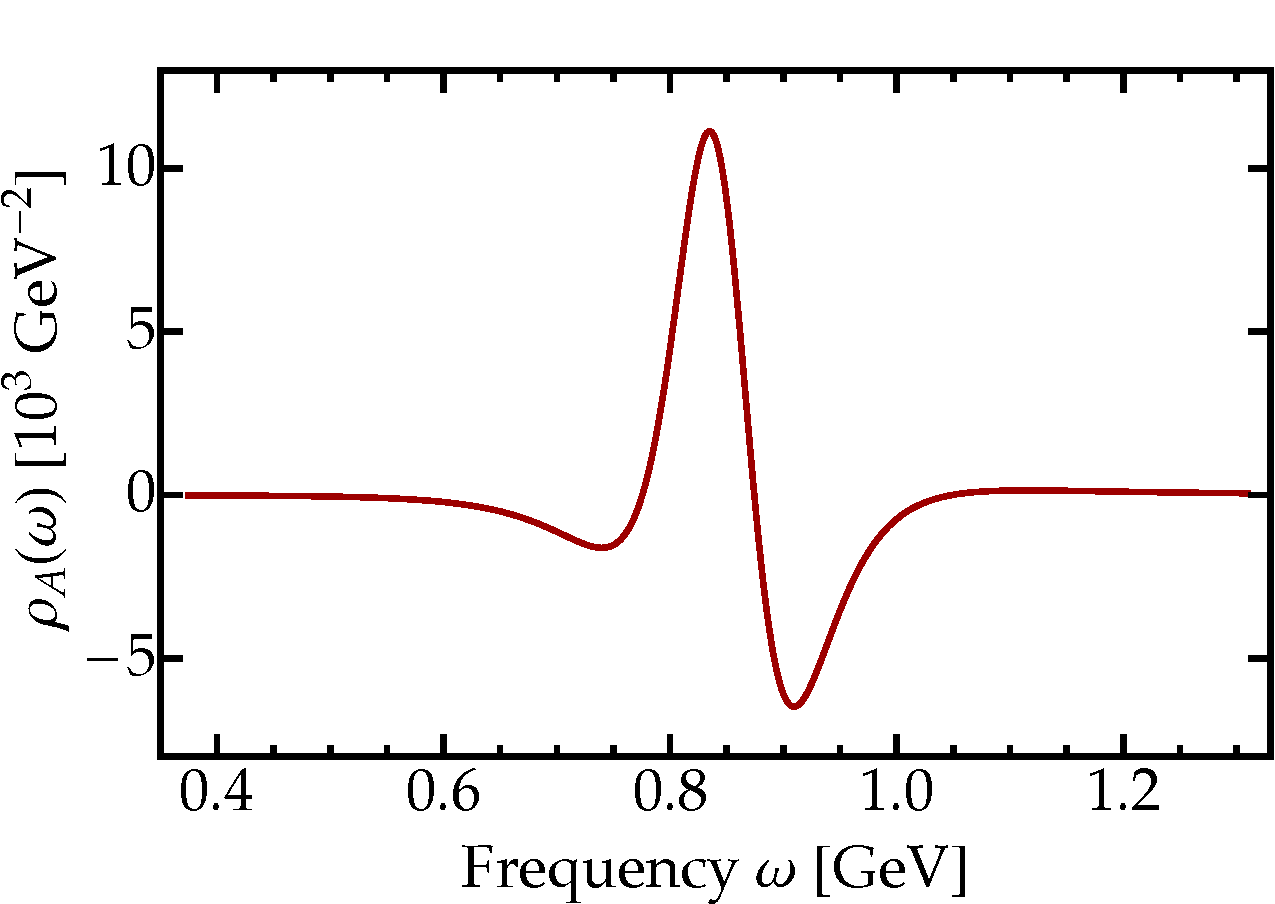
\includegraphics[width = 0.46\textwidth, trim= 4em 0 0 0]{figs/plots/GluonSpecFuncPlot}
\hfill
	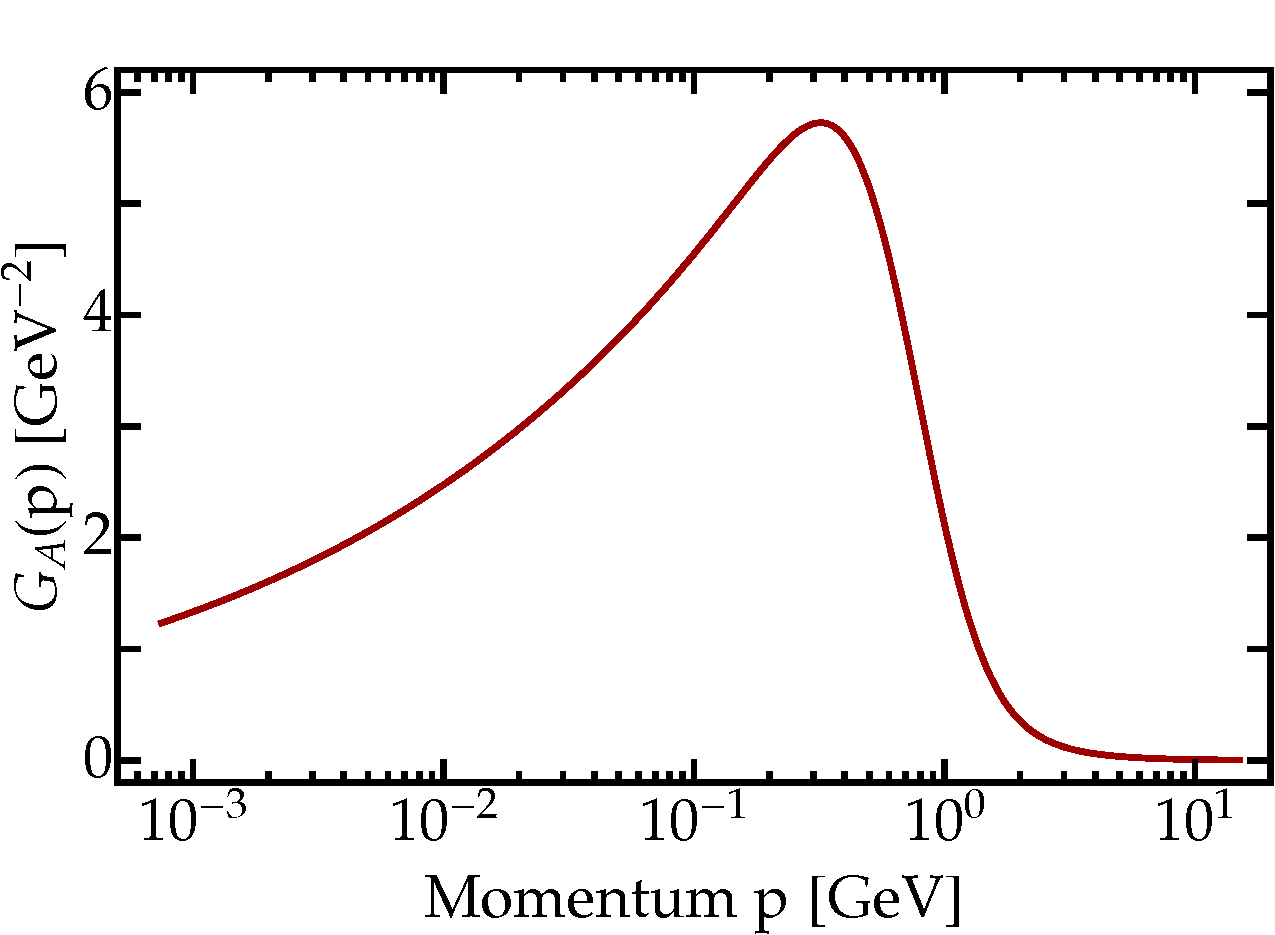
\includegraphics[width = 0.445\textwidth, trim= 4em 0 0 0]{figs/plots/GluonPropPlot}
\hfill
	\caption[Chosen input gluon spectral function and corresponding propagator.]{Chosen input gluon spectral function (left) and the corresponding propagator obtained from \eqref{eqn:GluonSpec} (right). This spectral function was determined in \cite{CyrolPawlowskiRothkopWink2018} by reconstructing numerical FRG data.}
\label{fig:gluon_specfunc_and_prop}
\end{figure}
This completes our presentation of the conducted calculations, the results for the spectral functions and all associated quantities are presented in the following section.

\section{Results and Implications}
This last section of the main part is devoted to the discussion of our results. The relevant quantities that are computed for every iteration step according to the iterative procedure presented in \figref{fig:numerics}, are the final expressions for the Dirac vector and scalar parts of the quark self energy diagram and the dressing functions $Z_q(p)$ and $M_q(p)$, that are accessed via the quark propagator DSE. Each of these quantities has been evaluated for Euclidean as well as real-time momenta/frequencies. The results shown in the following are obtained by interpolating the discrete expressions, that were obtained by computing the numerical integrals on a discrete momentum grid. Again, we refer to \appref{chap:appendixC} for further details concerning the numerical implementation. \\The results for the computed  dressing functions for different iteration steps are displayed in \figref{fig:computed_dressings}, at the beginning of the next page. Note, that the initially arbitrary momentum scales can be converted into actual physical units via the peak position of the input gluon spectral function, which has been determined in lattice studies to be at around 1 GeV. 
 Qualitatively, the results for the iterated dressing functions look very stable, already for a small number of iterations. The wave function renormalization tends to one in the IR and to zero in the UV with a rather smooth transition in the range from 10 to $10^2$ GeV. This specific form hints at a problem with the finiteness of the Dirac vector part in our computation. From its definition as $Z_q(p)=1/A(p)$, where $A(p)$ collects all parts of the quark DSE, that are $\sim i\slashed{p}$, it looks like the value of the Dirac vector part of the diagram tends to infinity, hence explaining the value of zero in $Z_q(p)$.  This problem could not be resolved yet upon completion of this thesis.\\
The quark mass function $M_q(p)$ also exhibits a stable IR and UV behavior, tending to a finite value of $\sim 0.38$ GeV in the IR. We observe a characteristic negative dip in the region of 1 GeV up to $10^2$ GeV, that should not be present, since the mass function should be a positive quantity. This could be related to the problem concerning $Z_q(p)$, which is also visible in the UV limit of the mass function where it tends to zero. This is expected from the properties of $Z_q(p)$, since it enters the computation of $M_q(p)=B(p)/A(p)=Z(p)B(p)$ as a multiplicative factor and therefore cancels out all non-zero contributions to $M_q(p)$ in the UV.
 \begin{figure}[t] 
\hfill
	\centering
	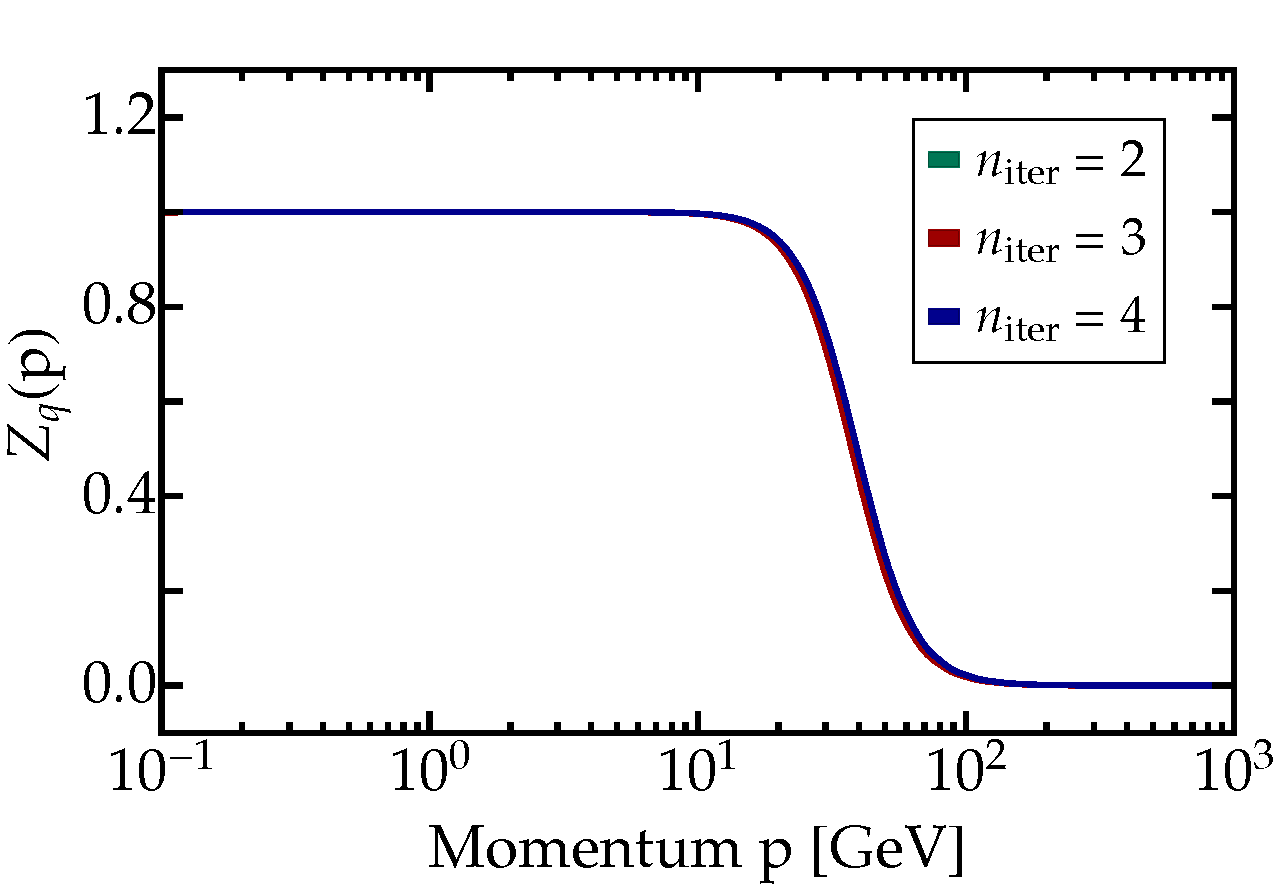
\includegraphics[width = 0.46\textwidth, trim= 4em 0 0 0]{figs/plots/ZqPlot}
\hfill
	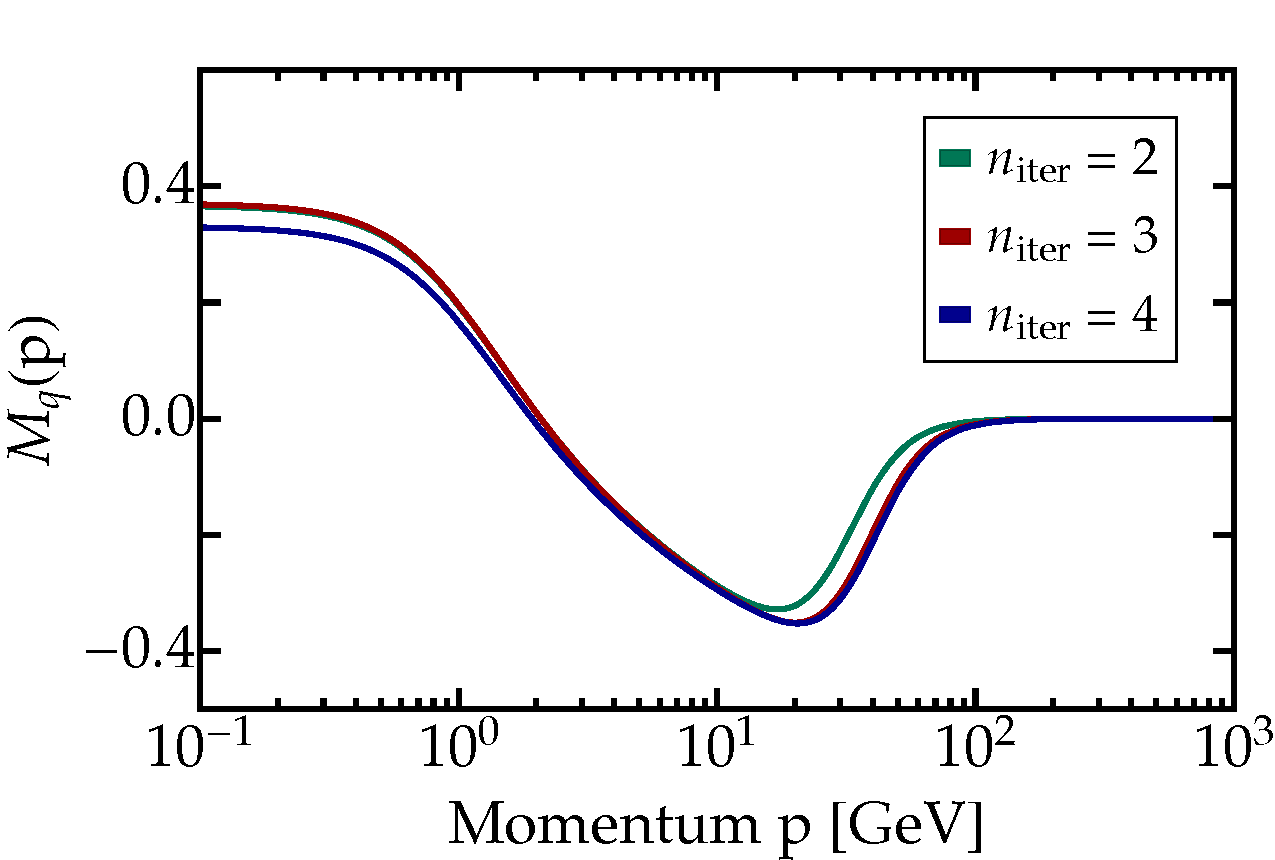
\includegraphics[width = 0.475\textwidth, trim= 4em 0 0 0]{figs/plots/MqPlot}
\hfill
	\caption[Computed quark propagator dressings $Z_q(p)$ and $M_q(p)$.]{Computed quark propagator dressings $Z_q(p)$ and $M_q(p)$ for different iteration steps.}
\label{fig:computed_dressings}
\end{figure}

The results for the quark spectral functions $\rho_q^D(\omega)$ and $\rho_q^M(\omega)$ are displayed in \figref{fig:specfunc_results} at the beginning of the next page. The development of the typical peak structure is clearly visible. The spectral functions feature negative regions, which might at first seem to be in contradiction with the probabilistic interpretation discussed in \chapref{chap:methods}. Upon further consideration however, this is also observed in other scenarios, such as for example for the gluon input we are using in this work. A possible explanation could be, that the two spectral functions associated with the quark propagator are no spectral functions of an actual observable particle and therefore are not necessarily required to obey positivy.  Nevertheless, no convergent solution for the iterative procedure could be found. As a benchmark check, we show the corresponding parts of the Euclidean propagator computed directly from the DSE, highlighted in blue, and from the spectral functions via \eqref{eqn:correct_relation}, highlighted in red. No exact agreement is observed and hence, the spectral representation is violated. This is another hint at a possible problem with the used input for the iterative procedure. Note, that as soon as the spectral representation is violated, the iterative solution procedure immediately breaks down, as \eqref{eqn:correct_relation} no longer holds. Starting from the above set of input parameters, the iteration runs into an unstable direction where the spectral representation does not hold for the quark propagators. To conclude this discussion we remark, that if there exists a solution to the quark DSE respecting the spectral representation, the initial conditions have to be closer to the actual solution, i.\,e. in the basin of attraction. Additionally, the observed discrepancies hint at an error in the calculation of the relevant diagram, that was not found  upon completion of this thesis. 
 
 \begin{figure}[t] 
\hfill
	\centering
	\includegraphics[width = 0.48\textwidth, trim= 4em 0 0 0]{figs/plots/rhoqDPlot}
\hfill
	\includegraphics[width = 0.48\textwidth, trim= 4em 0 0 0 0]{figs/plots/rhoqMPlot}
\hfill \\
\hfill
	\centering
	\includegraphics[width = 0.485\textwidth, trim= 3em 0 0 0]{figs/plots/BenchmarkPlotVec}
\hspace{0.5em}
	\includegraphics[width = 0.485\textwidth, trim= 3em 0 0 0]{figs/plots/BenchmarkPlotScal}
\hfill
	\caption[Computed quark spectral functions $\rho_q^D(\omega)$ and $\rho_q(\omega)$ and corresponding propagator dressings.]{First row: Computed quark spectral functions $\rho_q^D(\omega)$ and $\rho_q^M(\omega)$ for different numbers of iterations. Second row: Comparison of the respective parts of the Euclidean quark propagator with the result obtained by the spectral representation given in \eqref{eqn:QuarkSpecFunc} for the last iteration step $n_{\mathrm{iter}}=4$.}
\label{fig:specfunc_results}
\end{figure}


	%\include{content/04_finiteT}
	
	
	
	
	\chapter{Conclusions and Outlook}\label{chap:conclusion}
In this thesis, we investigated quark spectral functions and the analytical properties of the associated real-time correlation functions by iteratively solving the corresponding Dyson-Schwinger equation in a novel approach based on the manifestly gauge-invariant dimensional regularization scheme.\\
After introducing the required background knowledge on functional approaches to QFT in \chapref{chap:methods}, and on the non-perturbative sector of QCD in \chapref{chap:qcd}, we introduced the central functional relations in the context of this work, the Dyson-Schwinger equations for the gluon, ghost and the quark propagators, the latter one being the relevant equation to set up our computation. In \chapref{chap:results}, we presented the application of the spectral renormalization scheme at the concrete example of the quark self energy diagram, as the non-trivial one-loop contribution to the quark propagator DSE. By naive power counting, the diagram is superficially divergent, which left us with the task to employ an appropriate regularization scheme in order to guarantee finite integrands . After regularizing the usual loop-momentum integration via dimensional regularization and the application of a BPHZ-type subtraction scheme in order to modify the UV-behavior of the integrands, we were left with finite expressions for the spectral integrands $I_q^D(p)$ and $I_q^M(p)$. The final step before being able to solve the quark DSE, was to analytically continue the obtained expressions to real-time frequencies, since the spectral functions are obtained from the imaginary parts if the respective parts of the retarded quark propagator. Based on this setup, a procedure to iteratively solve the quark DSE by employing an initial ansatz for the quark spectral functions $\rho_q^D$ and $\rho_q^M$, that allows for a numerical treatment of the remaining spectral integrals, was put forward. For the input gluon spectral function we used an analytic result, that has been reconstructed from numerical data for the Euclidean quark propagator. In every iteration step, the quark DSE is solved and an updated result for the spectral functions was obtained, that served as input for the next iteration steps.\\
In the considered approximation, replacing the full 3-point vertex by the respective classical, bare counterpart and employing a quasi-classical ansatz for the quark spectral functions to initialize the iterative procedure, no convergent solution of the quark DSE could be obtained up to now. The development of the typical peak structure could indeed be observed for $n_{\mathrm{iter}}>2$, but the mandatory benchmark test, the comparison between the characteristic parts of the Euclidean quark propagator computed directly via the DSE and from the respective spectral functions, shows no exact agreement.
As we have seen, the current setup did not yet suffice to produce stable results. Additional work is therefore required to upgrade the numerical setup to ensure convergence of the iterative procedure. In addition, it would also be very important to examine the possibilities of choosing different initial conditions, first of course for the quarks, but also for the gluonic input, as done for example in  \cite{HorakPapavassiliouPawlowskiWink2021} for the spectral ghost DSE, where the impact of a whole range of slightly different gluon input spectral functions was studied. 
After finishing the computation in the classical vertex approximation it would be of course desirable to include the full vertex, as it naturally appears in the DSE . This of course complicates the computation, since another spectral representation, i.\,e. for the quark-gluon vertex, needs to be included in the calculation  of the one-loop digram and therefore another spectral integration needs to be performed for every iteration step.  \\ % TODO: Refer to refs
On longer terms, we want to extend our results to finite temperatures and densities. This can for example be examined within thermal field theory approaches such as the Matsubara formalism \cite{Matsubara1955}, where the momentum integration in the time  domain $p^0$ is replaced by a discrete sum over the respective Matsubara frequencies, giving rise to the usual quantum statistical distribution functions, that directly depend on temperature and chemical potential. This is currently studied in a scalar theory setting in our group. \\
One possibility for improvements on the numerical side, especially if we wish for faster iteration times, would be to discretize the spectral integrands on a three-dimensional grid (in the $p/\omega-\lambda_1-\lambda_2$ parameter space) and interpolate the obtained data points. In comparable studies this leads to faster iteration times of up to two orders of magnitude, cf. the appendix of \cite{HorakPapavassiliouPawlowskiWink2021}. Our current setup takes around four to seven hours to perform a single iteration.\\
Of course, the general aim of our project line is to have a precise knowledge of the spectral properties of all relevant QCD quantities. Once this is achieved, this  can be used to study and make predictions for various interesting QCD phenomena such as the dynamics of the quark-gluon plasma in relativistic heavy-ion collisions whose evolution is usually described in terms of hydrodynamical transport equations.

\cleardoublepage



%Appendices
\begin{appendices}
	\chapter{Detailed Calculation of the Quark Self Energy}\label{chap:appendixA}
This first appendix is denoted to the technical details of the conducted calculations. In order to obtain the final expression  for the quark self energy diagram $\Sigma_q(p)$, we need to perform three different integrations, i.\,e. the ususal integration over the loop momentum $q$, the Feynman parameter $x$, introduced to facilitate the momentum integration, and finally the integration over the spectral parameters $\lambda_1$ and $\lambda_2$, respectively. We will highlight the most important steps of each part of the calculation and present the full analytical expressions in the end.\\
The Feynman rules for QCD in the Landau gauge can be derived from \eqref{eqn:S_QCD}, they are summarized for example in the appendix of \cite{NPgaugeLecture}. 


\section*{General Tensor Structure and Manipulations}
 The relevant diagram for our computation of the quark spectral function is the one-loop contribution to the Dyson-Schwinger equation for the (inverse) quark propagator:
\begin{align}
\bigg(\includegraphics[scale=0.4, valign=c]{figs/diagrams/quarkDSE/full_quark_propagator}\bigg)^{-1} = 
\bigg(\includegraphics[scale=0.4, valign=c]{figs/diagrams/quarkDSE/bare_quark_propagator.pdf}\bigg)^{-1} - \includegraphics[scale=0.4, valign=c]{figs/diagrams/quarkDSE/quark_self_energy}
\end{align}
 Applying the Feynman rules for QCD in the Landau gauge  we find\footnote{Note, that we work in a classical vertex approximation, i.\,e. $\Gamma^{(3)}_{q\bar{q}A} \equiv S^{(3)}_{q\bar{q}A}$, as discussed in the main part. This explains the replacement of the red blob in this explicit visualization.}:
\begin{align*}
\includegraphics[scale=0.45, valign=c, trim = 0 6em 0 0]{figs/diagrams/quark_self_energy_classical} := \Sigma_q
(p) &= (-ig)^2 \delta^{ab}C_f \int_q\ \Pi^{\mu\nu}_{\perp}(q) G_A(q)\gamma_{\mu}G_q(p+q)\gamma_{\nu},
\end{align*}
with the transverse projection operator $\Pi^{\mu\nu}_{\perp}(q)$ as defined in (\ref{eqn:transversal_projector}). \\

For the gluon and quark propagators, we insert the respective  K\"all\'{e}n-Lehmann spectral representations, i.\,e.
\begin{align} 
G_A(q)&=\int_{\lambda_1} \frac{\lambda_1\rho_A(\lambda_1)}{q^{2}+\lambda_1^{2}},
\end{align}
and
\begin{equation}
\begin{aligned}
G_q(p+q) = \left(\slashed{p} + \slashed{q}\right) \int_{\lambda_2} \frac{\lambda_2\rho_{q}^D(\lambda_2)}{(p+q)^{2}+\lambda_2^2}+\int_{\lambda_2} \frac{\lambda_2\rho_q^M(\lambda_2)}{(p+q)^{2}+\lambda_2^2}.
\end{aligned}
\end{equation}
For a detailed discussion of the Dirac structure of the quark propagator we refer to \appref{chap:appendixB}. \\
The structure of the quark propagator allows us split the computation of the full diagram into two components, its Dirac vector and scalar part, i.\,e.
\begin{equation}
	\Sigma_q(p) =\slashed{p}\cdot\Sigma_{q}^D(p) + \Sigma_{q}^M(p).
\end{equation}
Whereas the scalar part $\Sigma_{q}^M(p)$ does not contain any additional gamma matrices, we have to be very careful when permuting the tensor structure of the vector part $\Sigma_{q}^M(p)$, where an additional gamma matrix is inherently implemented via $\slashed{p}= p^{\alpha}\gamma_{\alpha}$. To be able to contract the Dirac indices of the transversal propagator with the two uncontracted indices of the vertices, we need to take care of the following, well known identities, cf. \cite{PeskinSchroeder1995}:
\begin{align}
\left\{\gamma_{\alpha},\gamma^{\nu}\right\} &= 2\delta_{\alpha}^{\phantom{{\alpha}}\nu}, \\
\gamma_{\mu}\gamma^{\mu} &= d, \\
\slashed{p}^2 &= p^2.
\end{align}
After carefully permuting all relevant terms we are left with:
\begin{equation}
	\begin{aligned}
		\slashed{p}\cdot\Sigma_{q}^D(p) &\sim \int_q \left((3-d)\slashed{p} + \left(\color{MScRed}(1-d)\normalcolor - \color{MScGreen}2\ \frac{p\cdot q}{q^2}\normalcolor\right)\slashed{q}\right)\int\limits_{\left\{\lambda_1,\lambda_2\right\}} \frac{\lambda_1\rho_A(\lambda_1)}{q^2 + \lambda_1^2} \frac{\lambda_2\rho_q^D(\lambda_2)}{(p+q)^2 + \lambda_2^2}, \\[0.5em]
		\Sigma_{q}^M(p) &\sim \int_q\ (d-1)\int\limits_{\left\{\lambda_1,\lambda_2\right\}} \frac{\lambda_1\rho_A(\lambda_1)}{q^2 + \lambda_1^2} \frac{\lambda_2\rho_q^M(\lambda_2)}{(p+q)^2 + \lambda_2^2}.
	\end{aligned}
\end{equation}
The nontrivial contributions arising from above considerations are highlighted in red and green. In the following we will manipulate all terms individually from left to right. Note, that the first (uncolored) term of the vector part has the same momentum structure as the scalar part, up to prefactors. \\
In a first step the integration order $q\leftrightarrow\left\{\lambda_1,\lambda_2\right\}$ is swapped, which is only allowed for finite integrands, according to Fubinis theorem. We already explained how to resolve this issue in the main part of this work, for an overview cf. \figref{fig:spectral_renormalization}. \\ Introducing Feynman parameters according to 
\begin{equation}
\frac{1}{A B}=\int_{0}^{1} \dd x\ \frac{1}{x A+(1-x) B},
\end{equation}
allows us to recast the first term as follows:
\begin{equation}
	(3-d)\slashed{p} \int_q \frac{1}{q^2 + \lambda_1^2}\frac{1}{(p+q)^2 + \lambda_2^2} = (3-d)\slashed{p}\int_{x,q} \frac{1}{\left[q^2 + \Delta_1\right]^2},
\end{equation}
where we defined
\begin{equation}
	\Delta_1 = x(1-x)p^2 + (1-x)\lambda_1^2 + x\lambda_2^2,
\end{equation}
and shifted the loop momentum $q \rightarrow q-xp$. As observed above, the same holds for the Dirac scalar part $\Sigma_{q}^M(p)$, the only difference is the prefactor of $(d-1)$. \\
 The term highlighted in red is a bit trickier since it involves another factor of $q^{\alpha}$ that is affected by the shift of the loop momentum: 
\begin{equation}
\begin{aligned}
	(1-d)\gamma_{\alpha} \int_q q^{\alpha} \frac{1}{q^2 + \lambda_1^2}\frac{1}{(p+q)^2 + \lambda_2^2} &= (1-d)\gamma_{\alpha}\int_{x,q} (q^{\alpha} - xp^{\alpha})\frac{1}{\left[q^2 + \Delta_1\right]^2}\\
	&= (d-1)\slashed{p}\int_{x,q}\frac{x}{\left[q^2 + \Delta_1\right]^2}.
	\end{aligned}
\end{equation}
In the last line we used the fact, that all integrations involving an odd power of $q$ in the numerator are zero.\\
 Following the same line of arguments, we can also simplify the third relevant term, highlighted in green. It features additional factors of $p$ and $q$ and an additional contribution to the denominator:
\begin{equation}
	\begin{aligned}
		-2\gamma_{\alpha} \int_q q^{\alpha}\frac{p\cdot q}{q^2} \frac{1}{q^2 + \lambda_1^2}\frac{1}{(p+q)^2 + \lambda_2^2} = -2\frac{\gamma_{\alpha}p_{\beta}}{\lambda_1^2}\int_q\left\{\left(\frac{ q^{\alpha}q^{\beta}}{q^2 ((p+q)^2 + \lambda_2^2)}\right)\right.\\ \left. - \left(\frac{ q^{\alpha}q^{\beta}}{(q^2 + \lambda_1^2)((p+q)^2 + \lambda_2^2)}\right)\right\}.
	\end{aligned}
\end{equation}
We decomposed the first part of the integrand using partial fraction decomposition,
\begin{equation}
\frac{1}{q^{2}} \frac{1}{q^{2}+\lambda_1^{2}}=\frac{1}{\lambda_1^{2}}\left(\frac{1}{q^{2}}-\frac{1}{q^{2}+\lambda_1^{2}}\right),
\end{equation}
in order to reduce the complexity of the denominator. Now we can again perform the Feynman trick and shift the loop momentum $q\rightarrow q-xp$ to obtain
\begin{equation}
	\cdots = -2\frac{\gamma_{\alpha}}{\lambda_1^2}\int_{x,q}\left\{ \left((p\cdot q)q^{\alpha} + x^2p^2p^{\alpha}\right)\left(\frac{1}{\left[q^2 + \Delta_2\right]^2} - \frac{1}{\left[q^2 + \Delta_1\right]^2}\right) \right\},
\end{equation}
where we again discarded all terms that were odd in $q$. Additionally we define
\begin{equation}
	\Delta_2 = \Delta_1 - (1-x)\lambda_1.
\end{equation}
In the first part of this expression we symmetrize the momenta according to 
\begin{equation}
	q^{\alpha}q^{\beta} = \frac{1}{d}\delta^{\alpha\beta}q^2,
\end{equation}
which is valid under the integral, and therefore find in total:
\begin{equation}
	\cdots = -2\frac{\slashed{p}}{\lambda_1^2}\int_{x,q}\left\{\frac{1}{d}\left(\frac{q^2}{\left[q^2 + \Delta_2\right]^2} - \frac{q^2}{\left[q^2 + \Delta_1\right]^2}\right) + p^2x^2\left(\frac{1}{\left[q^2 + \Delta_2\right]^2} - \frac{1}{\left[q^2 + \Delta_1\right]^2}\right)\right\}
\end{equation}
To condense our notation, we sort the contributions to both parts of the diagram in  powers of $q^2$ and collect the prefactors as coefficients $A_i$, $B_i$ and $C_i$. This concludes the first part of the calculation and renders the loop momentum integration trivial. We arrive at
\begin{align}
\Sigma_{q}^D(p) &= (-ig)^2\delta^{ab}C_f\int\limits_{\left\{\lambda_1,\lambda_2\right\}}\lambda_1\lambda_2\rho_A(\lambda_1)\rho_q^D(\lambda_2)\cdot I_q^D\left(p, \lambda_1, \lambda_2,x\right),\\
\Sigma_{q}^M(p) &= (-ig)^2\delta^{ab}C_f\int\limits_{\left\{\lambda_1,\lambda_2\right\}}\lambda_1\lambda_2\rho_A(\lambda_1)\rho_q^M(\lambda_2)\cdot I_q^M\left(p, \lambda_1, \lambda_2,x\right),
\end{align}

with the respective integrands defined as
\begin{align}
I_q^D\left(p, \lambda_1, \lambda_2,x\right)&=\int_{q, x} \sum_{i=0}^{1}\left(q^{2}\right)^{i}\left[\frac{A_{i}}{\left[q^{2}+\Delta_{1}\right]^{2}}-\frac{B_{i}}{\left[q^{2}+\Delta_{2}\right]^{2}}\right],\\
I_q^M\left(p, \lambda_1, \lambda_2,x\right)&=\int_{q, x} \sum_{i=0}^{1}\left(q^{2}\right)^{i}\left[\frac{C_{i}}{\left[q^{2}+\Delta_{1}\right]^{2}}\right],
\end{align}
and the  coefficients are given by
\begin{equation}
\begin{alignedat}{3}
&A_0 = \frac{2p^2x^2}{\lambda_1^2}+ 3x -1,   \qquad  &&B_0 = \frac{2p^2x^2}{\lambda_1^2},    \qquad       &&C_0 = 3, \\
&A_1 = \frac{1}{2\lambda_1^2},  			 \qquad  &&B_1 = \frac{1}{2\lambda_1^2},          \qquad  	  &&C_1 = 0. \\
\end{alignedat}
\end{equation}
Note, that the presented coefficients are already evaluated in $d=4$, we explicitly checked, that they do not change when going to $d=4-2\varepsilon$ and performing the limit $\varepsilon\rightarrow 0$, which will be discussed in more detail in the subsequent section.

\section*{Loop Momentum Integration}
In this form, the momentum integration can be performed using standard integration formulae known in the context of dimensional regularization, the regularization scheme of our choice. The respective integrals are solved via
\begin{equation}
	\int\frac{\dd^d q}{(2\pi)^d}\frac{(q^2)^m}{\left[q^2 + \Delta\right]^n} = \frac{1}{(4\pi)^{d/2}}\frac{\Gamma(m+\frac{d}{2})\Gamma(n-\frac{d}{2}-m)}{\Gamma(\frac{d}{2})\Gamma(n)} \Delta^{m+d/2-m},
\end{equation} 
with $m$ a non-negative and $n$ a positive integer \cite{PeskinSchroeder1995}. For our computation the relevant expressions have $n=2$ and $m= 0,1$. Explicitly, the term with $m=0$ evaluates to
\begin{equation}
\begin{aligned}
	\int \frac{\dd^d q}{(2\pi)^d} \frac{1}{\left[q^2 + \Delta\right]^2} &\overset{\phantom{(*)}}{=}  \frac{1}{(4\pi)^{\frac{d}{2}}} \frac{\Gamma(2-\frac{d}{2})}{\Gamma(2)} \Delta^{\frac{d}{2}-2} \\
	&\overset{(*)}{=} \frac{1}{(4\pi)^{2}}\left(\frac{1}{\varepsilon} - \operatorname{log}\Delta - \gamma_{\mathrm{E}} + \operatorname{log} 4\pi + \operatorname{log} \mu^2 + \mathcal{O}(\varepsilon)\right)\\
	&\overset{\phantom{(*)}}{=} \frac{1}{(4\pi)^{2}}\left(\frac{1}{\varepsilon} - \operatorname{log}\Delta + \operatorname{log}\left(\frac{4\pi\mu^2}{\operatorname{e}^{\gamma_{\mathrm{E}}}}\right)   + \mathcal{O}(\varepsilon)\right),
	\end{aligned}
\end{equation}
where we evaluate for $d= 4 -2\varepsilon$ and expand the relevant quantities up to lowest order in the limit $\varepsilon\rightarrow 0$. Note, that to account for this change in the dimensionality, we introduced a factor of $\mu^{2\varepsilon}$ under the integral. Here, $\Gamma(n)$ is the usual gamma function and  $\gamma_{\mathrm{E}}\approx 0.57722$ is the Euler-Mascheroni constant.\\ This isolates the divergence of the diagram in the $\frac{1}{\varepsilon}$-term, which is discarded, as usual. Note, that as a remnant of swapping the integration order we are not done yet and still need to renormalize the spectral integrands appropriately. The second important integral ($n=2$ and $m=1$) is solved analogously:
\begin{equation}
\begin{aligned}
	\int \frac{\dd^d q}{(2\pi)^d} \frac{q^2}{\left[q^2 + \Delta\right]^2} &=  \frac{1}{(4\pi)^{\frac{d}{2}}} \frac{\Gamma(1+\frac{d}{2})\Gamma(1-\frac{d}{2})}{\Gamma(\frac{d}{2})\Gamma(2)} \Delta^{\frac{d}{2}-1} \\
	&= \frac{1}{(4\pi)^{\frac{d}{2}}}\left(\frac{d}{2-d}\right)\Gamma\big(2-\frac{d}{2}\big) \Delta\cdot\Delta^{\frac{d}{2}-2} \\
	&= \frac{-2}{(4\pi)^{2}}\Delta\left(\frac{1}{\varepsilon} +\frac{1}{2}- \operatorname{log}\Delta - \gamma_{\mathrm{E}} + \operatorname{log} 4\pi + \operatorname{log} \mu^2 + \mathcal{O}(\varepsilon)\right)\\
	&= \frac{-2}{(4\pi)^{2}}\Delta\left(\frac{1}{\varepsilon} +\frac{1}{2} - \operatorname{log}\Delta + \operatorname{log}\left(\frac{4\pi\mu^2}{\operatorname{e}^{\gamma_{\mathrm{E}}}}\right)   + \mathcal{O}(\varepsilon)\right),
	\end{aligned}
\end{equation}
where we used the properties of the gamma function, $\Gamma(z+1)=z\Gamma(z)\ \forall z\in \mathbb{C}$.\\

Reordering the expression in powers of the Feynman parameter $x$, we arrive at:
\begin{align}
I_q^D\left(p, \lambda_1, \lambda_2\right) &=\left(\frac{1}{\varepsilon}+\log \left(\frac{4 \pi \mu^{2}}{e^{\gamma_{\mathrm{E}}}}\right)\right) \sum\limits_{i=0}^{2}\left( \frac{\alpha_{i}-\beta_{i}}{i+1}\right) - \frac{1}{4}\nonumber\\
&-\mathlarger{\int}_{x} \sum\limits_{i=0}^{2} x^{i}\left(\alpha_{i} \log \Delta_{1}-\beta_{i} \log \Delta_{2}\right)   + \mathcal{O}(\varepsilon) \label{eqn:IqD}\\[0.5em]
I_q^M\left(p, \lambda_1, \lambda_2\right)&=\left(\frac{1}{\varepsilon}+\log \frac{4 \pi \mu^{2}}{e^{\gamma_{\mathrm{E}}}}\right) \gamma_0
-\mathlarger{\int}_{x} \gamma_{0} \log \Delta_{1} +\mathcal{O}(\varepsilon).\label{eqn:IqM}
\end{align}


We will present the full analytical expressions for the coefficients and integrals on the next pages. Note, that the prefactor of $1/(4\pi)^2$ is pulled out of the integrand in order to replace $\alpha = g^2/(4\pi)$ in the global prefactor.

\section*{Feynman Parameter Integration}
In the next step, the respective Feynman integrals can be performed. We use standard Mathematica integration routines and compare the results of the explicit integrations with  numerical integration as a benchmark check. The relevant integrals are  
\begin{align}
	f_i(p,\lambda_1, \lambda) &\sim \int_0^1 \dd x\ x^{i} \operatorname{log}\Delta_1 \\
g_i(p,\lambda_1, \lambda) &\sim \int_0^1 \dd x\ x^{i} \operatorname{log}\Delta_2 \\
h_0(p,\lambda_1, \lambda) &= \int_0^1 \dd x\ \operatorname{log}\Delta_1
\end{align}
with $i$ ranging from 0 to 2. The lengthy expressions are displayed on the next pages, together wit the reordered coefficients introduced above.\\ This completes the first major part of the calculation, we now need to focus on the renormalization of the the obtained expressions in order to access the final result for the spectral integrands, that serve as an input to our iterative procedure. 

\afterpage{%
\newgeometry{width=180mm,top=3cm}
\begin{landscape}
	\begin{center}
		\newcommand{\col}[1]{\label{eq:coeff_A_#1}\qquad\qquad}
\newenvironment{titledeqns}[1]{\large\bfseries{#1}
}{}

\newcommand{\tunedvs}{3pt}

\makeatletter 
\def\leqno{\tagsleft@true}\def\reqno{\tagsleft@false} 
\makeatother 

\leqno

\hspace{0pt}
%\vspace{1em}
\begin{titledeqns}{Coefficients and Explicit Expressions for the Feynman Parameter Integration - Dirac Vector Part I}
%\vfill
\begin{align}
 \alpha_0 &= -2, \\[1em]
\alpha_1 &= -\frac{p^2+\lambda_2^2 - 4\lambda_1^2}{\lambda_1^2}, \\[1em]
\alpha_2 &= \frac{3p^2}{\lambda_1^2}, \\[3em]
f_0 &= \frac{1}{p^2}\left[\left(\lambda_1^2-\lambda_2^2\right)  \operatorname{log} \left(\frac{\lambda_2}{\lambda_1}\right)+\zeta\cdot \operatorname{arcoth}\left(\frac{\lambda_2^2+\lambda_1^2+p^2}{\zeta}\right)\right] + \operatorname{log} (\lambda_2)+ \operatorname{log} (\lambda_1)-2, \\[1em]
f_1 &=  \frac{1}{4 p^4}\left[-\mathcal{D}_{\mathrm{cut}}\cdot\zeta\left(\lambda_2^2-\lambda_1^2+p^2\right) -2 p^2 \left(\lambda_2^2-\lambda_1^2+2 p^2\right)+2 \operatorname{log} (\lambda_2) \left(-\left(\lambda_2^2-\lambda_1^2\right)^2-2 \lambda_2^2 p^2+p^4\right)  \right. \\ &\hspace{3.81em}+2 \left. \operatorname{log} (\lambda_1) \left(-2 \lambda_2^2 \lambda_1^2+\lambda_1^4+\left(\lambda_2^2+p^2\right)^2\right)\right],\notag \\[1em]
 f_2 &= \frac{1}{18 p^6}\left[-\mathcal{D}_{\mathrm{cut}}\cdot 3\zeta \left(\lambda_1^4-\lambda_1^2 \left(2 \lambda_2^2+p^2\right)+\left(\lambda_2^2+p^2\right)^2\right) -p^2 \left(6 \left(\lambda_2^2-\lambda_1^2\right)^2+3 p^2 \left(5 \lambda_2^2-\lambda_1^2\right)+13 p^4\right)  \right. \\ &\hspace{3.81em}+6 \left.\operatorname{log} (\lambda_2) \left(-\left(\lambda_2^2-\lambda_1^2\right)^3+3 \lambda_2^2 p^2 \left(\lambda_1^2-\lambda_2^2\right)-3 \lambda_2^2 p^4+p^6\right)  \right.\notag \\ &\hspace{3.81em}+6 \left. \operatorname{log} (\lambda_1) \left(\lambda_2^2-\lambda_1^2+p^2\right) \left(\lambda_1^4+\lambda_1^2 \left(p^2-2 \lambda_2^2\right)+\left(\lambda_2^2+p^2\right)^2\right)\right], \notag
\end{align}
\end{titledeqns}
%\vfill

		\end{center}
\vspace{-2em}
where we defined
		\begin{align*}
\mathcal{D}_{\mathrm{cut}} = \operatorname{log} \left(\zeta - \lambda_1^2+\lambda_2^2-p^2\right)-\operatorname{log} \left(\zeta -\lambda_1^2 +\lambda_2^2+p^2\right)+\operatorname{log} \left(\zeta +\lambda_1^2-\lambda_2^2-p^2\right)-\operatorname{log} \left(\zeta +\lambda_1^2 -\lambda ^2+p^2\right),
\end{align*}	
with
\begin{equation*}
	\zeta=\sqrt{\lambda_1^{4}+\left(\lambda_2^{2}+p^{2}\right)^{2}+2 \lambda_1^{2}\left(p^{2}-\lambda_2^{2}\right)}.
\end{equation*}	

\begin{center}
		\pagebreak

\newcommand{\col}[1]{\label{eq:coeff_A_#1}\qquad\qquad}
\newenvironment{titledeqns}[1]{\large\bfseries{#1}
}{}

\newcommand{\tunedvs}{3pt}

\makeatletter 
\def\leqno{\tagsleft@true}\def\reqno{\tagsleft@false} 
\makeatother 

\leqno

\hspace{0pt}
\vspace{2em}
\begin{titledeqns}{Coefficients and Explicit Expressions for the Feynman Parameter Integration - Dirac Vector Part II}
\begin{align}
 \beta_0 &= 0,  \\[1em]
 \beta_1 &= -\frac{p^2+\lambda_2^2}{\lambda_1^2}, \\[1em]
 \beta_2 &= \frac{2p^2}{\lambda_1^2}, \\[3em]
 g_0 &= \frac{\lambda_2^2 \operatorname{log}\left(\frac{p^2}{\lambda_2^2}+1\right)}{p^2}+ \operatorname{log}\left(\lambda_2^2+p^2\right)-2, \\[1em]
 g_1 &=\frac{\left(\lambda_2^2+p^2\right)^2  \operatorname{log} \left(\lambda_2^2+p^2\right)-\left(\lambda_2^2+2 p^2\right) \left(2 \lambda_2^2  \operatorname{log} (\lambda_2)+p^2\right)}{2 p^4},\\[1em]
 g_2 &= -\frac{15 \lambda_2^2 p^4+6 \lambda_2^4 p^2+12  \operatorname{log} (\lambda_2) \left(\lambda_2^6+3 \lambda_2^4 p^2+3 \lambda_2^2 p^4\right)-6 \left(\lambda_2^2+p^2\right)^3  \operatorname{log} \left(\lambda_2^2+p^2\right)+13 p^6}{18 p^6}. \end{align}
\vspace{2em}
\end{titledeqns}

\begin{titledeqns}{Coefficients and Explicit Expressions for the Feynman Parameter Integration - Dirac Scalar Part}
\begin{align}
 \gamma_0 &= 3, \\[1em]
 h_0 &= f_0 = \frac{1}{p^2}\left[\left(\lambda_1^2-\lambda_2^2\right)  \operatorname{log} \left(\frac{\lambda_2}{\lambda_1}\right)+\zeta\cdot \operatorname{arcoth}\left(\frac{\lambda_2^2+\lambda_1^2+p^2}{\zeta}\right)\right] + \operatorname{log} (\lambda_2)+ \operatorname{log} (\lambda_1)-2. 
\end{align}
\end{titledeqns}

\reqno
		\end{center}	
\end{landscape}
\clearpage
\restoregeometry
}
\newpage
\section*{Renormalization of the Spectral Integrands}
The renormalization of the spectral integrands according to a BPHZ-scheme has already been discussed in great detail in the main part of this work. The general idea is to cancel the quadratic and logarithmic divergencies of the different parts of the diagram by subtraction of a Taylor expansion in all momenta about the renormalisation scale $\mu$, resulting in finite integrands in the limit $\varepsilon\rightarrow 0$.
Here, we just want to show some exemplary plots to visualize the effects of the subtraction procedure on different parts of the Dirac vector integrand $I_q^D(p)$.
 \begin{figure}[H] 
 \centering
	\begin{minipage}{0.8\textwidth}
		\includegraphics[width = 0.88\textwidth]{figs/plots/FiniteIntegrands1}
	\end{minipage}
	\begin{minipage}{0.8\textwidth}
		\includegraphics[width = 0.88\textwidth]{figs/plots/FiniteIntegrands2}
	\end{minipage}\caption[Effects of the BPHZ-type subtraction on the integrands, exemplary shown for logarithmically and quadratically divergent parts of the spectral integrand of the Dirac vector part.]{Effects of the BPHZ-type subtraction on the integrands, exemplary shown for logarithmically and quadratically divergent parts of the spectral integrand of the Dirac vector part, cf. \eqref{eqn:IqD}. The other parameters in this plot are fixed to $p=1$ GeV, $\mu = 2$ GeV and $\lambda_1=1$. We checked the effects for various combinations, these specific values were just chosen for demonstration purposes.}
	\label{fig:BPHZ_demonstration}
\end{figure}



\section*{Going to Real Frequencies}
In order to obtain real-time expressions for the computed quantities, we need to evaluate (\ref{eqn:IqD}) and (\ref{eqn:IqM}) at real frequencies, i.\,e. 
\begin{equation}
	I_q^{(D/M)}\left(\omega, \lambda_1, \lambda_2\right) := I_q^{(D/M)}\left(-i(\omega + i0^+)\right).
\end{equation}
 From the definitions of the functions $\alpha_i, \beta_i$ and $\gamma_i$, and $f_i, g_i$ and $h_0$, their respective real-time counterpart is trivially obtained by the substitution $p\leftrightarrow -i\omega$. This is again done in Mathematica, employing the convention $\operatorname{Im}\operatorname{log} x = \pi$\ for $x<0$ for the logarithmic branch cut. 
As a proof of concept, we show that the real-time expression of the Dirac vector part $I_q^{D}\left(\omega\right)$ is in agreement with the expression obtained by explicitly taking the correct limit $\varepsilon\rightarrow 0^+$. We show the real and imaginary parts of  $I_q^{D}\left(-i(\omega + i0^+)\right)$ for different finite values of $\varepsilon$ ranging from $10^{-1}$ to $10^{-5}$ in comparison with the corresponding real-time expression of the diagram $I_q^{D}\left(\omega,\lambda_1,\lambda_2\right)$ in \figref{fig:continuation}.
 \begin{figure}[t] 
\hfill
	\centering
	\includegraphics[width = 0.465\textwidth, trim= 4em 0 0 0]{figs/plots/ReContCheck}
\hfill
	\includegraphics[width = 0.52\textwidth, trim= 0 0.2em 0 0]{figs/plots/ImContCheck}
\hfill
\caption{Real and imaginary parts of the real-time expression $I_q^{D}\left(\omega,\lambda_1,\lambda_2\right)$ in comparison with the correct limit $\varepsilon\rightarrow 0^+$ for different finite values of $\varepsilon$.}
	\label{fig:continuation}
\end{figure}

\section*{Spectral Integrations}
The last step of the calculation consists of performing the (numerical) spectral integrals. With our obtained results for the Euclidean as well as the Minkowski expressions of the regularized integrands at hand, the only missing ingredients are the spectral functions for the gluon and the quarks. In order to be able to perform the spectral integration, appropriate initial \enquote{guesses} for both quark spectral functions $\rho_q^D(\lambda_2)$ and $\rho_q^M(\lambda_2)$ have to be made. In principle, the same would also apply to the gluon spectral function $\rho_A$, but since we have access to an analytic expression for $\rho_A$ from \cite{CyrolPawlowskiRothkopWink2018}, cf. \figref{fig:gluon_specfunc_and_prop}, $\rho_A$ does not need to be updated for every iteration step. For the quarks, we employ quasi-classical spectral functions, reproducing  the classical, perturbative quark propagator
\begin{equation}
	G_q(p) = \frac{-i\slashed{p}+m_q}{p^2+m_q^2}.
\end{equation}
They are simply given by a Dirac delta distribution, rendering the first iteration step trivial. As discussed before, we have to pay attention to the fact, that we are working with a spectral function of a linear argument $\lambda$. We therefore have to be careful with the correct implementation of the Dirac delta distribution. For a composed  function, we know that
\begin{equation}
	(\delta\circ f)(x) = \sum_i^{N_{\mathrm{roots}}}\frac{\delta(x-x_i)}{\abs{f'(x_i)}},
\end{equation}
which implies for our specific case
\begin{equation}
	\delta(x^2-a^2) = \frac{1}{\abs{2a}}\delta(x-a).
\end{equation}
This results in the following expressions for the initially empleyed quark spectral functions:
	\begin{align}
		\rho_{q,\mathrm{init}}^D(\lambda) &= 2\pi i\ \frac{\delta(\lambda-m_q)}{2\lambda}\\
		\rho_{q,\mathrm{init}}^M(\lambda) &= 2\pi m_q\ \frac{\delta(\lambda-m_q)}{2\lambda}.
	\end{align}
This completes our discussion of the calculation of the quark self energy diagram (up to the numerical spectral integrations, that need to be performed in every iteration step for the updated results for the quark spectral functions). Further details on the numerical implementation can be found in \appref{chap:appendixC}.
	\chapter{Disentangling the Dirac Structure of the Quark Propagator}\label{chap:appendixB}
In this short appendix, we want to have a closer look at the Dirac structure of the quark propagator DSE, in order to understand how we can access the spectral functions associated with the respective parts of the (retarded) quark propagator. This additional structure, meaning that the quark DSE is matrix-valued, is the main difference compared to the scalar and ghost DSE analyzed in \cite{HorakPawlowskiWink2020} and \cite{HorakPapavassiliouPawlowskiWink2021}.
\section*{Inverting the Quark DSE to obtain the Quark Propagator}
As discussed in \chapref{chap:methods}, the full propagator $G(p)$ is the inverse of the 2-point function $\Gamma^{(2)}(p)$. In our specific case, the 2-point function for the quarks computed via the DSE reads
\begin{equation}
\begin{aligned}
		\Gamma^{(2)}_q(p) = G^{-1}_q(p) &= G_{q,0}^{-1}(p) - \Sigma_q(p) \\
		&= i\slashed{p} A(p) + B(p) \\
		&= \frac{1}{Z_q(p)}\left(i\slashed{p} + M_q(p)\right),
\end{aligned}
\end{equation}
featuring the bare inverse propagator $G_{q,0}^{-1}(p)$ and the one-loop quark self energy $\Sigma_q(p)$. In the second line, we introduce two scalar dressing functions $A(p)$ and $B(p)$, collecting all parts of the DSE that are proportional to either $i\slashed{p}$ or unity. We will refer to the different parts of the (inverse) propagator as Dirac vector ($\sim i\slashed{p}$) and Dirac scalar ($\sim \mathbb{1}$) part\footnote{We do not explicitly write a unit matrix next to the Dirac scalar part, its meaning as being proportional to unity in Dirac space should be implicitly understood.} in the following. For similar discussions in the context of QCD confer \cite{Solis2019} and in QED  confer \cite{JiaPennington2017}. 
It is a common choice to redefine the scalar dressings to $Z_q(p)$ and $M_q(p)$ instead, which are known as the quark wave function renormalization and the quark mass function. They are related to $A(p)$ and $B(p)$ via
\begin{equation}
	 Z_q(p) = \frac{1}{A(p)}\qquad \text{and}\qquad M_q(p) = \frac{B(p)}{A(p)}.
\end{equation}
The two dressing functions $Z_q(p)$ and $M_q(p)$ are known from perturbation theory, cf. \cite{PelaezTissierWschebor2014, BarriosGraceyPelaezReinosa2021}, lattice studies, cf. \cite{Parappilly2005,Parappilly2006}, and functional methods, cf. \cite{GaoPapavassiliouPawlowski2021}, and can therefore be compared to our results.\\
With this parameterization of the inverse quark propagator at hand, we can now explicitly perform the inversion to obtain the full expressions for the Dirac vector and scalar part of the quark propagator in terms of the dressing functions introduced before:
\begin{equation}
\begin{aligned}
	 G_q(p) &= Z_q(p)\left(\frac{1}{i\slashed{p} + M_q(p)}\right)  \\
		&= Z_q(p)\left(\frac{-i\slashed{p} + M_q(p)}{(i\slashed{p} + M_q(p))(-i\slashed{p} + M_q(p))}\right) \\
		&= Z_q(p)\left(\frac{-i\slashed{p} + M_q(p)}{p^2 + M_q^2(p)}\right) \\
		&= -i\slashed{p} \left(\frac{Z_q(p)}{p^2 + M_q^2(p)}\right) +  \left(\frac{Z_q(p)M_q(p)}{p^2 + M_q^2(p)}\right)\\
		&\equiv -i\slashed{p}\cdot G_q^D(p) + G_q^M(p).
\end{aligned} \label{eqn:quark_prop_inversion}
\end{equation}
Here we used the fact, that 
\begin{equation}
	\begin{aligned}
		\slashed{p}^2 = p_{\mu}p_{\nu}\gamma^{\mu}\gamma^{\nu} &= p_{\mu}p_{\nu}\big(\left\{\gamma^{\mu},\gamma^{\nu}\right\} - \gamma^{\nu}\gamma^{\mu}\big)\\
		&= p_{\mu}p_{\nu}\big(2\delta^{\mu\nu} - \gamma^{\nu}\gamma^{\mu}\big)\\
		&= 2p^2 - \slashed{p}^2,
	\end{aligned}
\end{equation}
and therefore $\slashed{p}^2 = p^2$. In the last line we labelled the Dirac vector and scalar part $G_q^D(p)$ and $G_q^M(p)$ , respectively.\\
Comparing the derived expression for the quark propagator with the spectral representation (\ref{eqn:QuarkSpecFunc}), allows for an identification of the spectral integrals involving $\rho_q^{D}(\lambda)$ and $\rho_q^{M}(\lambda)$ with the Dirac vector and scalar part of the propagator:
\begin{equation}
\begin{aligned}
	G_q(p) &=-i\slashed{p}\cdot G_q^D(p) + G_q^M(p)\\
	&\equiv \slashed{p} \int_\lambda\frac{\lambda\rho_q^{D}(\lambda)}{p^2+\lambda^2} + \int_\lambda\frac{\lambda\rho_q^M(\lambda)}{p^2+\lambda^2}.
	\end{aligned}\label{eqn:quark_prop_identification}
\end{equation}
In \chapref{chap:methods} we presented the relation between the spectral function and the retarded propagator, given by \eqref{eqn:specfunc_relation}. Since this relation is of pivotal importance for this work (and for the next steps of our considerations in this chapter), we present a detailed derivation in the following section. 

\section*{Accessing the Spectral Function(s) from the retarded Propagator}
To derive \eqref{eqn:specfunc_relation}, we explicitly perform the analytic continuation $p\rightarrow -i\left(\omega + i\varepsilon\right)$ and consider the limit $\epsilon\rightarrow 0^+$. The only modification in the spectral representation of the propagator occurs in the denominator, hence we can focus on this part of the expression: 
\begin{equation}
	\begin{aligned}
		\lim\limits_{\epsilon\rightarrow 0^+} \frac{1}{-(\omega + i\epsilon)^2 + \lambda^2} &= 	\lim\limits_{\epsilon\rightarrow 0^+} \frac{1}{-\omega^2 + \epsilon^2 + \lambda^2 - 2i\epsilon\omega} \\
		&= 	\lim\limits_{\epsilon\rightarrow 0^+} \frac{-\omega^2 + \epsilon^2 + \lambda^2 + 2i\epsilon\omega}{(\epsilon^2 + \lambda^2 - \omega^2)^2 + 4\omega^2\epsilon^2}
	\end{aligned}
\end{equation}
Focusing only on the imaginary part yields
\begin{equation}
	\begin{aligned}
		 \lim\limits_{\epsilon\rightarrow 0^+}  \Im\left[\frac{1}{-(\omega + i\epsilon)^2 + \lambda^2}\right] &= \lim\limits_{\epsilon\rightarrow 0^+}  \frac{2\epsilon\omega}{(\epsilon^2 + \lambda^2 - \omega^2)^2 + 4\omega^2\epsilon^2} \\
		&= \frac{1}{2\omega}  \lim\limits_{\epsilon\rightarrow 0^+} \frac{\epsilon}{\left(\frac{\epsilon^2 + \lambda^2 - \omega^2}{2\omega}\right)^2 + \epsilon^2}\\
		&= \frac{\pi}{2\omega}\delta\left(\frac{\lambda^2-\omega^2}{2\omega}\right) \\
		&= \frac{\pi}{2\omega}\left(\eval{\frac{\partial\left(\frac{\lambda^2-\omega^2}{2\omega}\right)}{\partial\lambda}}_{\lambda=\omega}\right)^{-1}\delta\left(\lambda-\omega\right)\\
		&= \frac{\pi}{2\omega}\delta\left(\lambda-\omega\right),
	\end{aligned}
\end{equation}
where we used the expression for the Fourier transform of the $\delta$-function and assumed $\omega > 0$ and $\lambda > 0$. In total we are left with:
\begin{equation}
	G(p) = \int_\lambda\frac{\lambda\rho(\lambda)}{p^2 + \lambda^2}\ \longrightarrow\ \int_\lambda\frac{\lambda\rho(\lambda)}{-\omega^2 + \lambda^2} + i\frac{\rho(\omega)}{2} = G\left(-i(\omega + i0^+)\right).
\end{equation}
From this it is clear that \eqref{eqn:specfunc_relation} holds:
\begin{equation}
	\rho(\omega) =  2 \operatorname{Im}\left[G\left(-i(\omega + i0^+)\right)\right].
\end{equation}
For our case (\ref{eqn:quark_prop_identification}) this means, that we can access the spectral functions after appropriately projecting on the Dirac vector and scalar part and making use of \eqref{eqn:specfunc_relation} afterwards.
This results in
\begin{align}
	\rho_q^D(\omega) &= 2 \operatorname{Im}\left[\Pi_{\slashed{p}} G_{q}\left(-i(\omega + i0^+)\right)\right] = 2 \operatorname{Im}\left[-i G_q^D(-i(\omega + i0^+))\right] \\
	\rho_q^M(\omega) &= 2 \operatorname{Im}\left[\Pi_{\mathbb{1}} G_{q}\left(-i(\omega + i0^+)\right)\right]  = 2 \operatorname{Im}\left[G_q^M(-i(\omega + i0^+))\right],
	\label{eqn:correct_relation}
\end{align}
where the respective projection operators $\Pi_{\slashed{p}}$ and $\Pi_{\mathbb{1}}$ are defined as
\begin{align}
	\Pi_{\slashed{p}}\left(\cdots\right) &= \operatorname{Tr}_{\mathrm{D}}\left[\frac{\slashed{p}}{p^2} \left(\cdots\right)\right],\\
	\Pi_{\mathbb{1}}\left(\cdots\right) &= \operatorname{Tr}_{\mathrm{D}}\left[\left(\cdots\right)\right].
\end{align}
Here, the index $\mathrm{D}$\ refers to the Dirac trace and we used the fact that the trace over an odd number of gamma matrices vanishes, cf. \cite{PeskinSchroeder1995}. This concludes our discussion on how to handle the Dirac structure of the quark propagator in the context of our work. To complete this appendix we will have a brief look at the determination of the poles of the quark propagator and the associated residues.
\section*{Finding Poles and computing the corresponding Residues}


To account for the the splitting  into pole and continuous contributions to the spectral functions, we need to compute the residue of the pole in every iteration step since it enters the pole contribution as a prefactor, characterizing the associated contour integral enclosing the (isolated) pole. The quark propagator has a natural pole, i.\,e. the zero crossing of the denominator of \eqref{eqn:quark_prop_inversion}, leading to a $\delta$-distribution in the spectral function. \\
We want to make use of the fact, that the residues of an inverse function can easily be computed, if we know the zeros of the original function, i.\,e.
\begin{equation}
	\text{If}\ f(a) = 0\ \text{is a first order root of}\ f \implies \operatorname{Res}_a \frac{1}{f} = \frac{1}{f'(a)},
\end{equation} 
for a complex function $f$ with $a\in\mathbb{C}$ \cite{Marshall2019}.
This translates in our case to
\begin{equation}
\begin{aligned}
	 \eval{p^2 + M_q^2(p)}_{p=p_{\mathrm{root}}} = 0 \implies \operatorname{Res}_{p_{\mathrm{root}}} G_q(p^2) &= \eval{\frac{1}{\partial_{p^2}\left(p^2 + M_q^2(p)\right)}}_{p=p_{\mathrm{root}}} \\ 
	 &=  \eval{\frac{1}{1 + 2M_q(p)\frac{\partial_pM_q(p)}{2p}}}_{p=p_{\mathrm{root}}}.
	 \end{aligned}\label{eqn:residue}
\end{equation}
In practice we use Mathematicas \texttt{FindRoot[]} method to find the correct pole position and apply \eqref{eqn:residue} to compute the corresponding residue after every iteration step.
	\chapter{Numerical Implementation in Mathematica}\label{chap:appendixC}
Since setting up the numerical framework for the conducted calculations was an integral part of this work, but is of course not reflected appropriately in this writeup, we want to give the interested reader a brief overview of the numerics developed in the scope of this thesis. All numerical calculations were performed in Mathematica \cite{Mathematica} equipped with FormTracer \cite{FormTracer}, a tool developed in our working group to trace large expressions, that are usually present in loop calculations in QFT.
\section*{Computation of the Self-Energy Diagram in the Quark DSE}
\begin{itemize}
	\item \footnotesize\url{https://github.com/mathieukaltschmidt/MSc-Thesis/Numerics/01_quarkDSE.nb}
\end{itemize}
In this notebook we perform the computation of the quark self-energy diagram, including a visualization of the respective renormalization procedure for the spectral integrals and cross checks for the analytic continuation of the obtained expressions.

\section*{Extracting the Spectral Function(s)}
\begin{itemize}
	\item \footnotesize\url{https://github.com/mathieukaltschmidt/MSc-Thesis/Numerics/02_SpecFuncIter.nb}
\end{itemize}
This notebook features the main part of the numerical work: We iteratively perform the numerical spectral integrals and access the quark spectral functions from the retarded propagator  by applying \eqref{eqn:specfunc_relation} and update the input spectral functions for every iteration step. For an overview of the code structure cf. \figref{fig:numerics}. Afterwards we perform some benchmark checks. \\
\newpage
\section*{Numerical Setup}
All numerical spectral integrations are performed in Mathematica using standard integration routines with a relative precision goal of $10^{-3}$. 
The spectral integrals are evaluated on discrete momentum grids and the resulting discrete expressions for the diagrams, the different dressings and the obtained spectral functions are interpolated using B-splines for the Euclidean, and Hermite polynomials for the Minkowski expressions.  This leaves us with continuous quark spectral functions, that are fed back into the computation after every iteration step.\\
In the following we summarize all important parameters of the iterative procedure in Table \ref{tab:numerical_input}.
\begin{table}[H]
\centering	
\begin{tabular}{Sl} \toprule
    {Parameter} & {Value} \\ \midrule
    $\alpha_s$  & 0.22  \\[0.5em] 
    $m_{q,0}$  & 1 MeV   \\[0.5em] 
    $\mu$  & 2 GeV   \\[0.5em] 
     \midrule 
    $\lambda_{1,\mathrm{min}}\ /\ \lambda_{2,\mathrm{min}}$  & $10^{-3}$\\[0.5em] 
    $\lambda_{1,\mathrm{max}}\ /\ \lambda_{2,\mathrm{max}}$  & $10^{2}$\\[0.5em]  
    $p_{\mathrm{min}}\  /\ \omega_{\mathrm{min}}$  & $10^{-2}$     \\[0.5em]  
    $p_{\mathrm{max}}\ /\  \omega_{\mathrm{max}}$  & $10^{3}$      \\[0.5em]  
    \bottomrule
\end{tabular}
\caption{Overview of all relevant parameters for the iterative procedure.}
\label{tab:numerical_input}
\end{table}
The three relevant external parameters that need to be fixed at the beginning are the quark mass parameter $m_{q,0}$, the strong coupling constant $\alpha_s$ and the RG scale $\mu$, i.\,e. the relevant scale  for the application of the spectral regularization. Note, that fixing the value of the strong coupling constant $\alpha_s$ is redundant, since it enters the diagram as a global prefactor that might be reabsorbed into the definition of the spectral function $\rho_q \rightarrow \sqrt{\alpha_s}\rho_q$. Here, it is set to the standard value of $\alpha_s=0.22$. 
 
	
	
	
\end{appendices}

\cleardoublepage

%References, Figures etc.
\thispagestyle{plain}
\addcontentsline{toc}{chapter}{References}
\nocite{*}
\printbibliography[title=References]
\cleardoublepage

{\hypersetup{linkcolor=black}
\pagenumbering{roman}
\addcontentsline{toc}{chapter}{List of Figures}
\listoffigures
\begingroup
\let\clearpage\relax
\listoftables
\addcontentsline{toc}{chapter}{List of Tables}
\endgroup
}	
\cleardoublepage
\addcontentsline{toc}{chapter}{Acknowledgements and Declaration of Authorship}
\thispagestyle{plain}
\makeatletter
\section*{Acknowledgements}
I guess for all of us the last year was very challenging in every way possible. Despite all the unfortunate circumstances I was lucky enough to be able to complete this important chapter of my life. This would not have been possible if I would not have had the right people around me. 
\begin{itemize}
	\item First and foremost I have to thank my supervisor Prof. Jan Pawlowski for allowing me again to join his amazing group and providing me with such an interesting project. Since the beginning of my Bachelor thesis about two years ago I had the pleasure to enjoy many discussions about physics and beyond with you that contributed greatly to my (not only) scientific knowledge.
	\item I also want to thank Prof. J\"org J\"ackel for agreeing to become the second referee for this thesis in the first place, but I am even more thankful for the time and effort he invested in helping me to find a suitable PhD project.
	\item My deepest gratitude belongs to  Jan Horak, not only for sharing his notes and giving advice concerning calculations and numerics but especially for always finding the time to discuss problems and for keeping me on track during all the ups and downs of the time in home office. It is due to him and his expertise that this project somehow succeeded in the end.
	\item I thank all members of the Strongly Correlated Systems Group for providing such a supportive and welcoming working environment and for all the meetings, game nights and pizza days, that kept the social spirit high during lockdown. I can only imagine how great this year would have been with all of you at the institute!
	\item For valuable comments on the transcript I want to thank  Fabian Glaser and Carl von Randow. Carl deserves an additional honorable mention for his incredible ability to spot even the tiniest code bugs and for his emotional support during many (late night) coding sessions, not only in the scope of this Master thesis. Additionally, I want to thank my dear friends Mercal Abdin and Marie Wintergerst that I can always rely on when it comes to proofreading and whenever I need them.	
	\item At this point I also want to thank Prof. Arthur Hebecker for his excellent lectures on various aspects of theoretical physics I had the pleasure to attend during my studies that built the foundation for developing my fascination for theoretical physics already in the early phases of my studies.
	\item As my studies come to an end I want to take the chance to thank my former high school teachers for arousing my interest in physics and mathematics that ultimately lead to the decision to study physics, a decision I have never regretted. Just to name the most influential ones I want to thank Josef Waltz for being such an inspiring math teacher,  Dr. Christopher B\"uhler who showed me how much fun it is to work on physics problems (even during examinations), Bj\"orn Lennartz for introducing me to many interesting aspects of physics in my last years of school and finally Michael J\"ulich for creating possibilities to discuss interesting topics beyond the scope of my studies, keeping me busy with challenging papers and for the possibility to share my passion for physics with his students for many years now.	
	\item Last but definitely not least, I thank my family and friends for all their support, confidence and time throughout the entire time of my studies. This includes of course my parents Marie-Paule und Bernd and my sister C\'{e}line, Ralf \& Bea, the original \enquote{Nobelpreistr\"ager} crew Alex, Benny, Berkay and Carl, who never failed to motivate and entertain me during lectures, exercise groups, endless exercise sheet sessions and beyond university since the first day of the preparation course and all other friends, no matter whether in Heidelberg or back home, that made the time of my studies so enjoyable.
\end{itemize}
\hfill
\thispagestyle{plain}
\section*{Declaration of Authorship}
I hereby certify that this thesis  has been composed by me and is based on my own work. \\
 Where I have consulted work of others it is always clearly attributed and where I have quoted work from others, the source is always given. With the exception of such quotations, this thesis is entirely my own work.    \\
 
Eppelheim, June 15th 2021 \hfill \rule{60mm}{.15mm} \par \vspace{-0.4em}
\hfill \@author
\vfill
\makeatother 
\addcontentsline{toc}{chapter}{Acknowledgements and Declaration of Authorship}

\end{document}��

